\documentclass[
	pdftex,
	a4paper,
	oneside,		% Einseitiger Druck.
	BCOR12mm,       % Bindekorrektur
	            	% Satzspiegel berechnen
	11pt,			% Schriftgroesse
	parskip=half,	% Halbe Zeile Abstand zwischen Absätzen.
	headsepline,	% Linie nach Kopfzeile.
	%abstracton,	% Abstract Überschriften
	ngerman		    % Translator
]{scrreprt}

\usepackage{graphicx}
\usepackage{graphics}

% ermoeglicht \begin{Verbatim}[samepage=true] fuer besseres copy&paste von Beispieloutput bzw. Code.
\usepackage{fancyvrb}

\usepackage{scrhack}
\usepackage{listings}

\usepackage[headsepline,plainheadsepline]{scrpage2}
\pagestyle{scrheadings}
\ihead[\rightmark]{\rightmark} \chead[]{}
\ohead[\pagemark]{\pagemark} \cfoot[]{}

\automark{chapter}
\renewcommand{\chaptermark}[1]{\markright{\ #1}}



\newcommand{\pdftitel}{Hausarbeit: Evakuierung}
\newcommand{\autor}{Andre Lehnert und Marcell Salvage}
\newcommand{\arbeit}{Geosensornetze}

\usepackage[
	pdftitle={\pdftitel},
	pdfauthor={\autor},
	pdfsubject={\arbeit},
	pdfcreator={pdflatex},
	pdfpagemode=UseOutlines, % Beim Oeffnen Inhaltsverzeichnis anzeigen
	pdfdisplaydoctitle=true, % Dokumenttitel statt Dateiname anzeigen.
	pdflang=de,              % Sprache des Dokuments.
	bookmarks,               % PDF-Lesezeichen
    bookmarksopen=true,      % Lesezeichenbaum aufgeklappt...
    bookmarksopenlevel=1,    % ...um eine Ebene
    bookmarksnumbered=true,
    pdfusetitle,             % LaTeX-Titelei als Metainfo nehmen
    pdfstartpage={1},        % mit welcher Seite das PDF öffnen
    pdfstartview={FitH},
    hyperfootnotes=true,     % Links auf Fußnoten
    hyperindex=true,         % Indexeinträge verweisen auf Text
    linkbordercolor={0 1 1}, % Rahmenfarbe interne Links
    menubordercolor={0 1 1}, % Rahmenfarbe Literaturlinks
    urlbordercolor={1 0 0}   % Rahmenfarbe externe Links
]{hyperref}

%Zeilenumbruch und mehr
\usepackage[activate]{microtype}

% Unterschrift
%\usepackage{caption}

% Ohne das Package haben eps-Dateien bei mir nicht funktioniert
\usepackage{epstopdf, epsfig}

% Für Änderung des Spacings von Listen
\usepackage{enumitem}

\usepackage[ngerman]{babel}

%Ermögliche das Nutzen von Umlauten im Quelltext ohne \"<vokal>
\usepackage[utf8x]{inputenc}

%Inhaltsverzeichnis
\usepackage{tocloft}
\tocloftpagestyle{empty}

%Farben
\usepackage{color}
\definecolor{LinkColor}{rgb}{0,0,0.2}
\definecolor{ListingBackground}{rgb}{0.92,0.92,0.92}

%Zeilenumbruch und mehr
\usepackage[activate]{microtype}

% FloatBarrier verhindern, dass ein float (z.b. figure) daran vorbei angeordnet wird
\usepackage{placeins}

% Allgorithmen
\usepackage{algorithm}
\usepackage{algorithmic}

\usepackage{amssymb}

%Quellcode
\usepackage{listings}
\usepackage{caption}
\lstset{               	         
breaklines=true,                
breakatwhitespace=true,  
showspaces=true,
showstringspaces=false,
captionpos=b
}


% Auszeichnung von Inline-Code für Klassennamen etc.?
\newcommand{\inlcode}{\texttt}


\title{\textbf{Geosensornetze}\\WS 2013/2014}
\author{Hausarbeit von\\\autor}

\begin{document}

\parindent 0pt
\parskip 6pt

\maketitle
\tableofcontents
\parindent 0pt

\chapter{Einf\"uhrung}
\setcounter{page}{1}

%Soll ein Gebäude aufgrund einer Gefahrensituation evakuiert werden, so geschieht dies übli-cherweise über Hinweisschilder, die den Weg zum nächsten Notausgang weisen. Sobald jedoch der Weg zu einem der Notausgänge blockiert ist, kommt es zu unerwünschten Situationen. Eine dynamische Gebäudeevakuierung basierend auf mobilen Geräten und lokaler Kommunikation kann Abhilfe schaffen.  
%
%In dieser Aufgabe soll eine NetLogo-Umgebung zur Simulation einer dynamischen Gebäude-evakuierung entwickelt werden. Dazu sollen Agenten (Menschen mit mobilen Geräten) model-liert werden, die sich frei im Gebäude bewegen, Gefahrensituationen in ihrer Umgebung erfas-sen und benachbarte Agenten warnen. Notausgänge sollen als statische Sensorknoten model-liert werden, die Informationen über ihre Position und Passierbarkeit im Netz verteilen. Zur Lo-kalisierung der mobilen Endgeräte soll ein dezentraler Lokalisierungsalgorithmus implementiert werden. 
%Die Simulation sollte sowohl in einem abstrahierten Grundriss (keine Wände, zufällig verteilte Notausgänge), als auch in einem realen Grundriss (IKG Etage, Lichthof) durchgeführt werden

asdasdasd\cite{Amundson.}


asdasd

asdasdasd\cite{Jonathan.2004}

\section{Aufgabenbeschreibung}

Mit Hilfe der NetLogo-Simulationsumgebung \cite{Netlogo.1999}


\chapter{Simulationsumgebung}
\label{cha:simulationsumgebung}

Das Kapitel der Simulationsumgebung befasst sich mit den Eingabemöglichkeiten zur Anpassung der Simulationsparameter, sowie der konkreten Umsetzung der simulierten Welt, mit der Logik für die Notausgänge, der Personen, der Gefahrensituationen und dem Kommunikationsmodell.

Die Ausgangsbasis für die verwendeten Modelle und Protokolle stammen aus den erstellten Übungen zur Vorlesung Gensensornetze, sie wurden jedoch auf die Anforderungen der Hausarbeit adaptiert.


%%%%%%%%%%%%%%%%%%%%%%%%%%%%%%%%%%%%%%%%%%%%%%%%%%%%%%%%%%%%%%%%%%%%%%%%%%%%%%%%%
%%%%%%%%%%%%%%%%%%%%%%%%%%%%%%%%%%%%%%%%%%%%%%%%%%%%%%%%%%%%%%%%%%%%%%%%%%%%%%%%%


\section{Benutzerschnittstelle}
\label{sec:benutzerschnittstelle}

In diesem Abschnitt werden die Interaktions- und Konfigurationsmöglichkeiten mit der Simulationsumgebung erläutert. Abbildung \ref{fig:gui} stellt einen Ausschnitt des grafischen Interfaces von NetLogo da, anhand dessen die Erklärungen in den folgenden Abschnitten besser einzuordnen sind. 

\begin{figure}[!ht]
\centering
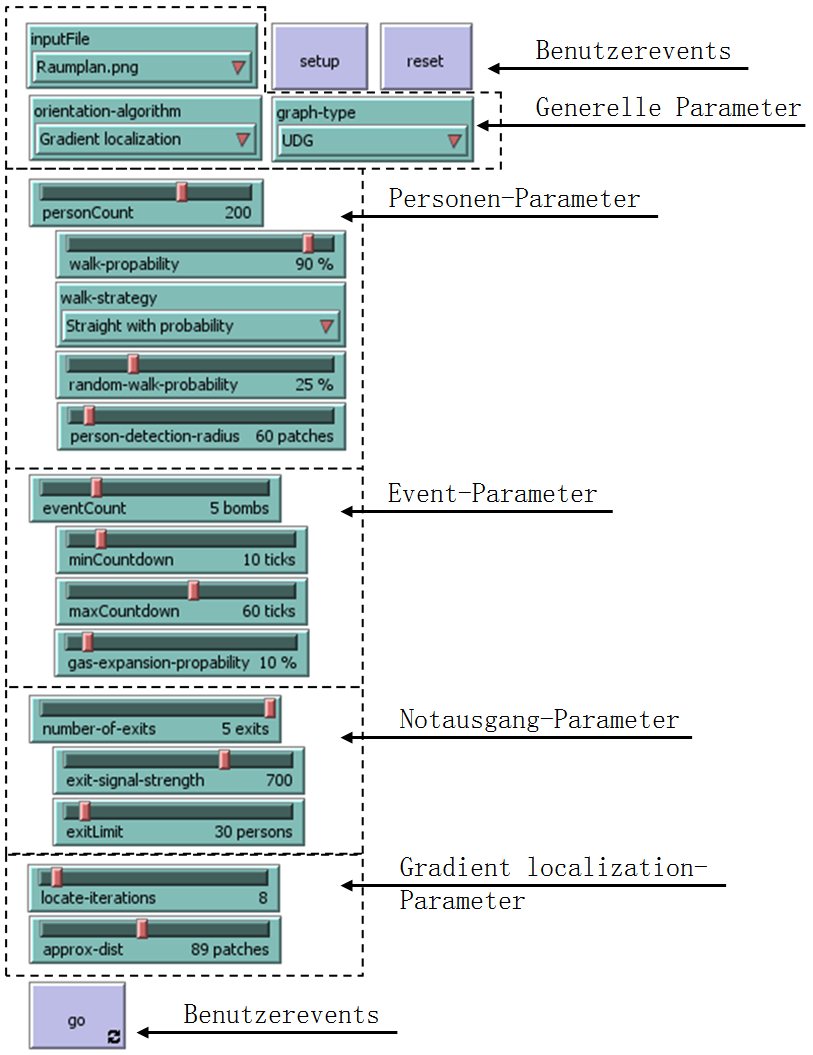
\includegraphics[height=0.85\textwidth]{simulationsumgebung/gui_3}
\caption{Grafische Oberfläche}
\label{fig:gui}
\end{figure}

\subsection{Benutzerevents}
\label{sec:gui_userevents}

Zum Auslösen von Benutzerevents werden Buttons verwendet. Zu diesen zählen \verb|setup|, \verb|reset| und \verb|go|, die hier kurz beschrieben werden.

\subsubsection*{setup-Button}

Die Betätigung des \verb|setup|-Buttons ruft eine Folge von Setup und Initialisierungsschritten auf. Zu Beginn wird die Simulationswelt erstellt. Dazu wird der Parameter \verb|inputFile| (siehe Abschnitt \ref{sec:gui_general}) zum Einbinden einer Bild-Datei und das Mapping der Pixel-Farbwerte auf die passend skalierte NetLogo-Welt gemappt. Das Ergebnis ist der gewählte Grundriss, bei dem jedes Patch einen Farbwert erhalten hat.

Dieser Farbwert ist essentiell für den nachfolgenden Schritt in der \verb|setup-patches|-Methode. Diese legt den Initialzustand jedes Patches fest (siehe Abschnitt \ref{sec:patches}). Generell wird auf Grund des Grundrisses zwischen leerem Raum (weiß) und einer Wand unterschieden (schwarz). 

Wände spielen auch bei der Initialisierung und Platzierung der Notausgänge eine wichtige Rolle, die mit der \verb|setup-exits|-Methode realisiert sind. Entsprechend der Aufgabenstellung werden Notausgänge auf einem abstrakten Grundriss, ohne Wände, zufällig in der Welt platziert. Für alle anderen Grundrisse mit Wänden wurde auf statische vordefinierte Positionen für Notausgänge gesetzt.\par
Bei der Initialisierung wird zudem die lokale Konstante der maximalen Signalreichweite für den Orientierungsalgorithmus \emph{cellular automaton} mit dem Parameter \verb|exit-signal-strength| aus Abschnitt \ref{sec:gui_exit} gesetzt und alle Notausgänge in den Zustand \emph{INIT} versetzt (vgl. Abschnitt \ref{sec:notausgaenge}).\par
Im Anschluss wird der \emph{cellular automaton}-Algorithmus (siehe Abschnitt \ref{sec:cellular_automaton}) ausgeführt, um die Patches mit Signalqualitätsinformationen auszustatten, damit die Personen den optimalen Fluchtweg bei einer Gefahrensituation nutzen.

Nachdem die Simulationswelt mit den statischen Elementen vorbereitet wurde, werden die Personen initialisiert und platziert. Dies geschieht mit der Methode \verb|setup-persons|. Hier wird eine definierte Anzahl von Personen erstellt (siehe Abschnitt \ref{sec:gui_person}, die auf einem abstrakten Grundriss zufällig und auf allen anderen zufällig mit einer Wand-Detektion platziert werden. Die Personen befinden sich nun im Zustand \emph{INIT} (vgl. Abschnitt \ref{sec:bewegungsmodell}).\par
Nach der Platzierung wird einmalig ein Kommunikationsgraph zwischen den Personen und den Notausgängen erstellt, damit der Nutzer ggf. den Graph-Typen oder die Kantenlänge anpassen kann (siehe Abschnitt \ref{sec:gui_person}).
 
Als letzter Schritt folgt die Initialisierung und Platzierung der Gefahrenevents  mittels \verb|setup-events|. Die analog zu den Personen auf dem abstrakten Grundriss zufällig und bei allen anderen Grundrissen mit Wand-Detektion platziert werden. Danach befinden sich alle Gefahrenevents im Zustand \emph{INIT} (vgl. Abschnitt \ref{sec:gefahrensituationen}).
 
\subsubsection*{reset-Button}

Mit dem \verb|reset|-Button werden alle definierten Parameter des letzten Setups wiederhergestellt und die Personen auf ihre ursprüngliche Position zurückgesetzt.
Ein fluten des Grundrisses ist nicht erforderlich und beschleunigt das durchführen von Messreihenreihen.
Zudem bietet es die Möglichkeit den Kommunikationsgraphen der Personen auszublenden, dies ist unter anderem nützlich bei der Darstellung der initial approximierten Positionen der Personen.

\subsubsection*{go-Button}

Schließlich kann die Simulation mit dem \verb|go|-Button gestartet und pausiert werden, da hier die \emph{forever}-Option aktiv ist. Ist diese deaktiviert, wird pro Betätigung des \verb|go|-Buttons nur ein \emph{Tick} durchgeführt.

\subsection{Generelle Parameter}
\label{sec:gui_general}

Der Parameter \verb|input-file| erlaubt die Definition des Grundrisses der Simulationsumgebung. Während des Setups wird der Parameter zur Pfadauflösung für eine Bild-Datei verwendet. Diese wird mit dem Befehl \verb|import-pcolors inputFile| auf die Simulationswelt gemappt.

\begin{quote}
\verb|input-file| $\in \{Abstract.png, Abstract\_static.png, Simple.png,$ \\\hspace*{2.6cm}$Raumplan.png\}$
\end{quote}

Der nächste generelle Parameter ist \verb|orientation-algorithm|. Dieser dient der Auswahl eines Algorithmus zur Orientierung und Lokalisierung der Personen. Detaillierte Informationen sind im Kapitel \ref{cha:algorithmik} aufgeführt.

\begin{quote}
\verb|orientation-algorithm| $\in \{Cellular$ $automaton, Gradient$ $localization\}$
\end{quote}

Mit dem \verb|graph-type|-Parameter hat der Nutzer die Wahl zwischen den Graphtypen, die in der Vorlesung vorgestellt wurden. Sofern \emph{UDG} gewählt ist, wird der \verb|person-detection-radius|-Parameter des folgenden Abschnitts für den Disk-Radius verwendet.

\begin{quote}
\verb|graph-type| $\in \{Complete$ $Graph, UDG, RNG, GG\}$
\end{quote}

\subsection{Personen--Parameter}
\label{sec:gui_person}

\verb|person-count| definiert die Anzahl der Personen in der Simulationsumgebung.

\begin{quote}
\verb|person-count| $\in [1, 300]$
\end{quote}

Mit dem \verb|walk-probability|-Parameter wird die Wahrscheinlichkeit definiert, mit der Personen bei einem Tick einen Schritt machen. Bei $0 \%$ werden die Personen statisch an der gegenwärtigen Position fixiert. Es ist also möglich diesen Parameter während der Laufzeit zu verändern.  

\begin{quote}
\verb|walk-probability| $\in [0, 100]$
\end{quote}

Der \verb|walk-strategy|-Parameter erlaubt die Auswahl der \emph{random walk}-Strategie (siehe Abschnitt \ref{sec:bewegungsmodell}).

\begin{quote}
\verb|walk-strategy| $\in \{Complete$ $random, Straight$ $with$ $collision$ $detection,$\\\hspace*{3.2cm}$Straight$ $with$ $probability\}$
\end{quote}

Analog zur \verb|walk-probability| kann der Nutzer den \verb|random-walk-probability|-Parameter zur Laufzeit anpassen und somit die Wahrscheinlichkeit der \emph{random walk} Richtungsänderung bestimmen. Bei $100 \%$ wird jede Person nach jedem Tick eine Richtungsänderung vornehmen.

\begin{quote}
\verb|random-walk-probability| $\in [0, 100]$
\end{quote}

Der \verb|person-detection-radius|-Parameter ist einer der entscheidendsten bei der Simulation. Hiermit wird der Radius definiert in dem eine Person eine Gefahrensituation wahrnehmen kann, sowie die Kommunikationsreichweite bei dem UDG-Graphen bestimmt. Zudem wird damit der Abstand zu einem Notausgang bestimmt (siehe Kapitel \ref{cha:algorithmik}.

\begin{quote}
\verb|person-detection-radius| $\in [0, 700]$
\end{quote}



\subsection{Event--Parameter}
\label{sec:gui_event}

Mit dem Parameter \verb|event-count| wird die Anzahl der zu platzierenden Gefahrenevents festgelegt. Bei \verb|event-count|$ = 0$ wird es zu keiner Gefahrensituation kommen, sodass der random-walk getestet werden kann.

\begin{quote}
\verb|event-count| $\in [0, 20]$
\end{quote}

In der Aufgabenstellung wird ein zufälliges Auslösen von Gefahrensituationen gefordert, die beiden Parameter \verb|min-countdown| und \verb|max-countdown| bewerkstelligen dies. Jedes einzelne Gefahrenevent erhält zufällig einen initialen Countdown im Intervall $[$\verb|min-countdown|, \verb|max-countdown|$]$. Die obere bzw. untere Intervallgrenze der Parameter wird durch den jeweils anderen Parameter eingeschränkt.  

\begin{quote}
\verb|min-countdown| $\in [1, $\textit{max-countdown}$]$
\end{quote}

\begin{quote}
\verb|max-countdown| $\in [$\textit{min-countdown}$, 100]$
\end{quote}

Der Parameter \verb|gas-expansion-probability| legt für alle Gefahrenevents die Ausbreitungswahrscheinlichkeit und somit die Ausbreitungsgeschwindigkeit fest. Bei $0 \%$ wird nur genau ein Patch unter dem jeweiligen Gefahrenevent zu einer Bedrohung für die Personen. Personen können die Gefahrensituationen somit wahrnehmen, die Wahrscheinlichkeit das Personen sterben ist jedoch sehr gering. 

\begin{quote}
\verb|gas-expansion-probability| $\in [0, 100]$
\end{quote}


\subsection{Notausgang--Parameter}
\label{sec:gui_exit}

Der Parameter zur Einstellung der verfügbaren Notausgänge in der simulierten Welt, 
\verb|number-of-exits| ist sehr bedeutsam bei der Lokalisierungsgenauigkeit und dem Fluchtverhalten der Personen.

\begin{quote}
\verb|number-of-exits| $\in [1, 9]$
\end{quote}

Zur dezentralen Orientierung der Personen und Schaffung eines optimalen Fluchtweges, wird auf den Zellulären Automaten zurückgegriffen und die Patches mit Informationen zur Signalstärke jedes Notausganges versehen.\par
Der Parameter \verb|exit-signal-strength| bildet die maximale Signalstärke bzw. Reichweite der Notausgänge ab. Es ist möglich, dass nicht jedes Patch mit allen Signalinformationen versehen ist, da die Reichweite eines Notausganges zu gering war.

\begin{quote}
\verb|exit-signal-strength| $\in [0, 1000]$
\end{quote}

Die Aufgabenstellung fordert eine Limitierung Fluchtkapazitäten von Notausgängen. D.h. Notausgänge können maximal \verb|exit-limit| Personen pro Tick evakuieren, sonst werden sie blockiert.

\begin{quote}
\verb|exit-limit| $\in [1, 300]$
\end{quote}

\subsection{Gradient localization--Parameter}
\label{sec:gui_localization}

- - - - - - - - - - - - - - - - - - - - - \\
TODO: Marcell Beschreibung der Parameter, Bedeutung\\
- - - - - - - - - - - - - - - - - - - - - \\

\verb|locate-iterations|

\begin{quote}
\verb|locate-iterations| $\in [0, 100]$
\end{quote}

\verb|approx-dist|

\begin{quote}
\verb|approx-dist| $\in [0, 200]$
\end{quote}





%%%%%%%%%%%%%%%%%%%%%%%%%%%%%%%%%%%%%%%%%%%%%%%%%%%%%%%%%%%%%%%%%%%%%%%%%%%%%%%%%
%%%%%%%%%%%%%%%%%%%%%%%%%%%%%%%%%%%%%%%%%%%%%%%%%%%%%%%%%%%%%%%%%%%%%%%%%%%%%%%%%

\section{Personen}
\label{sec:personen}

Personen sind Agenten, die mit NetLogo als \emph{breed} modelliert werden. Mit einem \emph{breed} kann das Konzept der Kapselung aus der Objektorientierung realisiert werden. Im Kontext einer Person können lokale Variablen deklariert werden, die von den abstrakten Variablen des \emph{breeds} vererbt werden. 

Mit diesem Konzept wird ein Lebenszyklus mit verschiedenen Zuständen und Zustandsübergängen für die Personen modelliert. 

% Lifecycle
\subsection{Lebenszyklus}

Der Lebenszyklus bestimmt das Verhalten der Personen. Die Zustände und die Zustandsübergänge werden in Abbildung \ref{fig:person} mittels eines Zustandsdiagramms beschrieben. 

Nach der Platzierung in der simulierten Welt befinden sich alle Personen im Zustand \verb|INIT|. In diesem Zustand wird ein \emph{random walk} ausgeführt. Die verschiedenen Typen werden im Abschnitt \ref{sec:bewegungsmodell} näher erläutert.

Nimmt eine Person in ihrem Sichtradius \verb|person-detection-radius| ein Gefahrenevent war, geht die Person in den Zustand \verb|EVENT_DETECTED| über. Hier versucht die Person andere Personen in der Umgebung zu warnen. Näheres ist dem Kommunikationsmodell im Abschnitt \ref{sec:kommunikationsmodell} zu entnehmen.

Nach dem Benachrichtigungsversuch wechselt die Person in den Zustand \verb|FLEEING|, bei dem die Person vor der Gefahrensituation flüchtet und versucht einen Notausgang zu erreichen. Zur Flucht wird ein anderes Bewegungsmodell verwendet, welches im Abschnitt \ref{sec:bewegungsmodell} beschrieben wird. Während der Flucht kann die Person weitere Gefahrensituation detektieren.

Erreicht die Person einen nicht blockierten Notausgang, ist sie gerettet und im Zustand \verb|RESCUED|. Die Person wird aus der Simulationsumgebung entfernt.

Bei einer Berührung mit dem Giftgas stirbt eine Person jedoch immer. Sie ist dann im Zustand \verb|DEAD|. Eine Interaktion ist mit ihr nicht mehr möglich. 

% INIT
% INIT, DEAD
% INIT, RESCUED
% INIT, EVENT_DETECTED, DEAD
% INIT, EVENT_DETECTED, FLEEING, RESCUED
% INIT, EVENT_DETECTED, FLEEING, DEAD

\begin{figure}
\centering
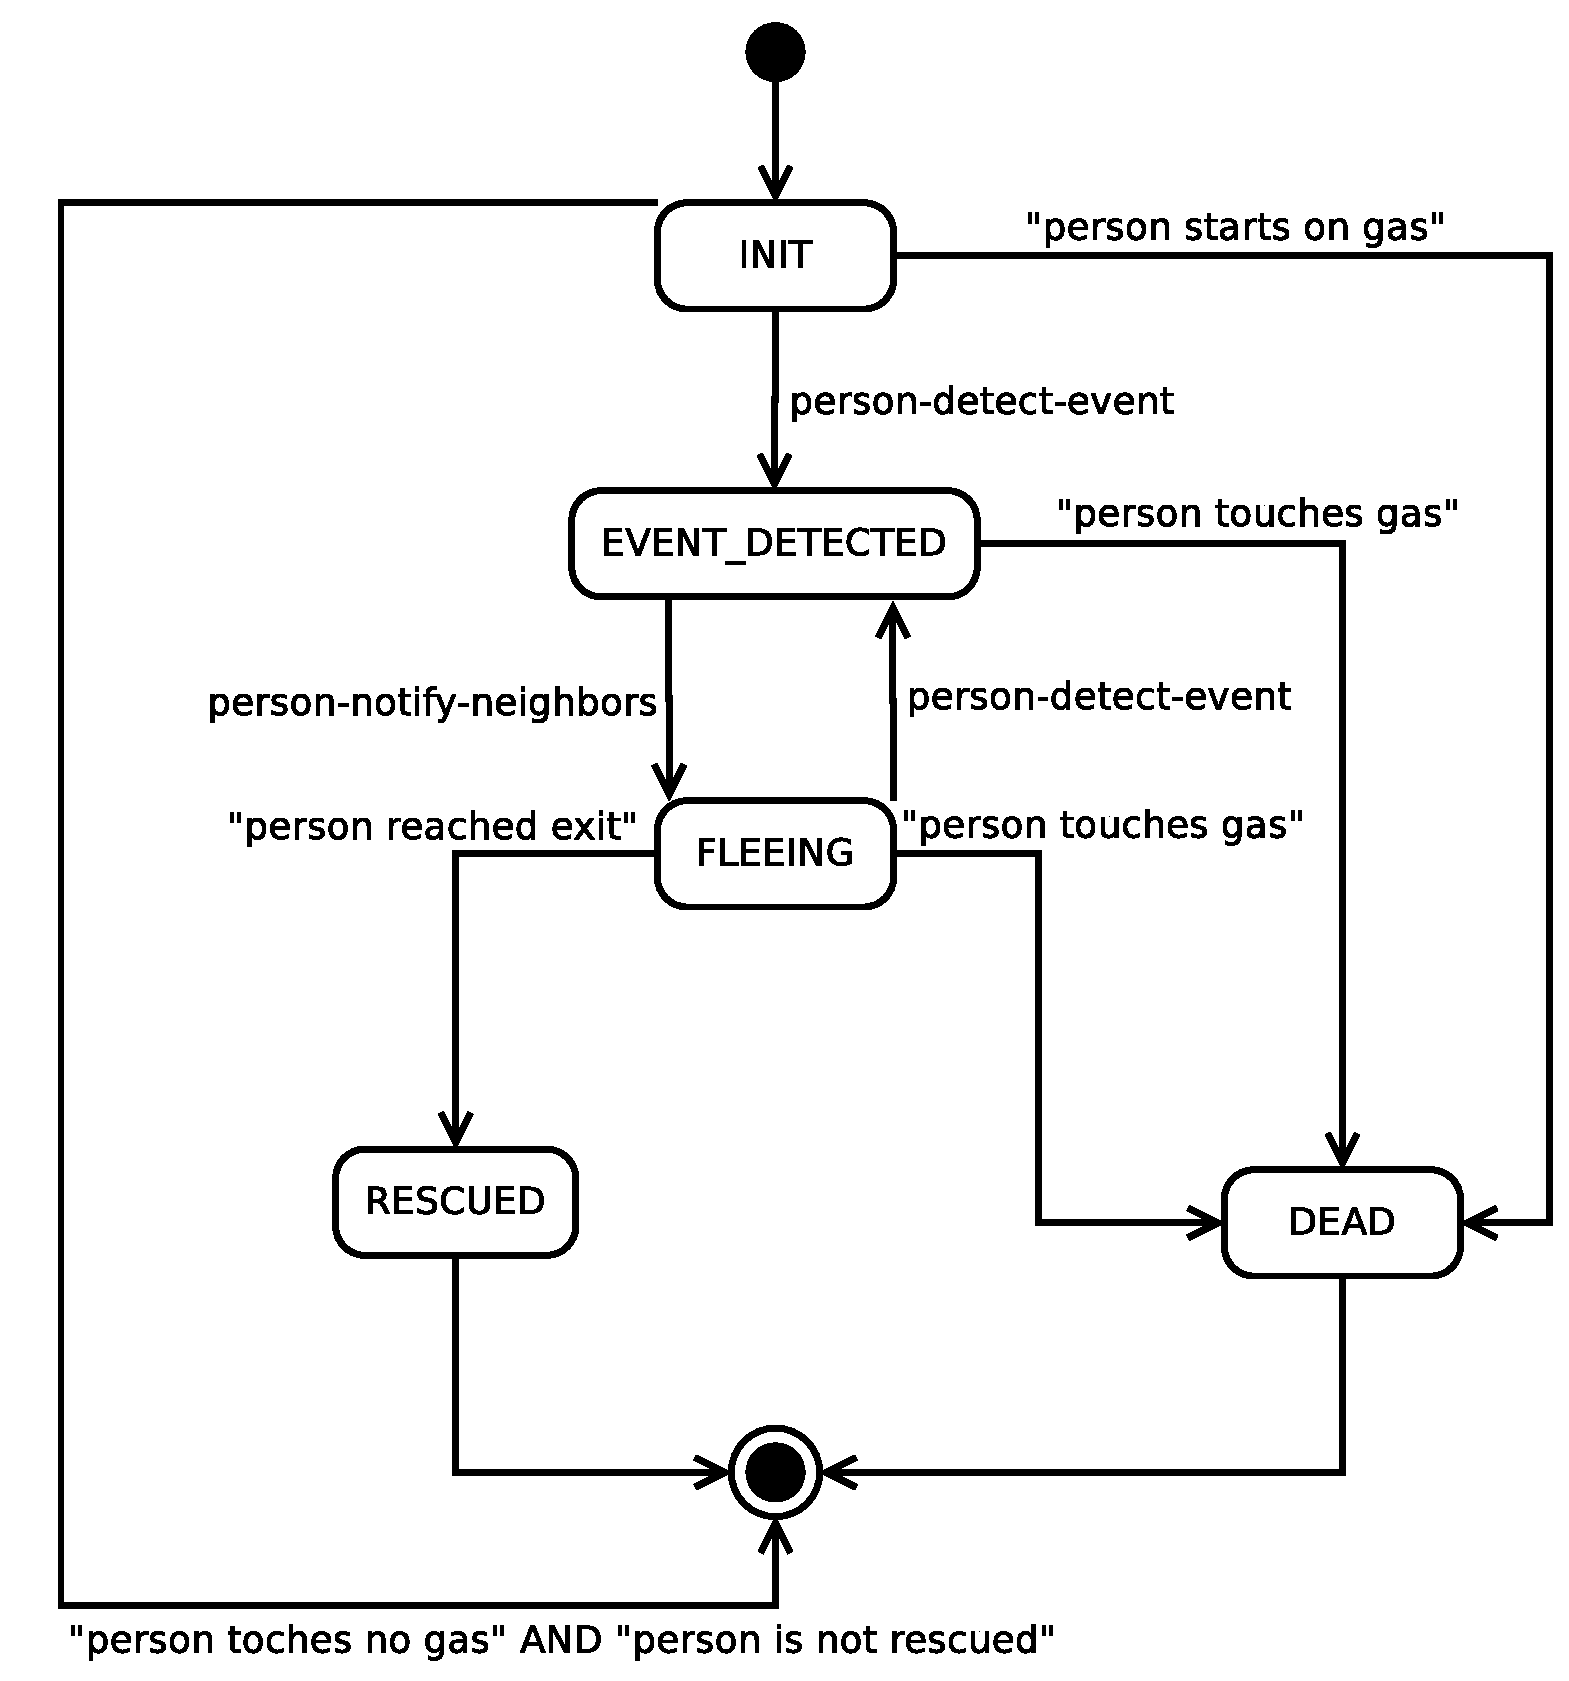
\includegraphics[height=0.6\textwidth]{simulationsumgebung/person.eps}
\caption{Zustandsdiagramm der Personen}
\label{fig:person}
\end{figure}

\subsection{Bewegungsmodell}
\label{sec:bewegungsmodell}
%Bewegungsmodell: Die Agenten sollen sich nach einem „Random Walk“ Modell bewegen. Agenten können Gefahren in ihrer Umgebung wahrnehmen und die Information an ihre nächs-ten Nachbarn weitergeben. Sobald ein Agent Informationen über eine Gefahrensituation hat, soll er sich auf dem kürzesten Weg zum nächsten Notausgang bewegen.  Hat ein Agent die Umgebung eines Notausgangs erreicht, soll er aus der Simulation genommen werden.

Für die Personen existieren zwei unterschiedliche Bewegungsmodelle, zum einen für Personen im \verb|INIT| Zustand und zum anderen für Personen im \verb|FLEEING| Zustand. Beide Modelle werden folgend erklärt.

\subsubsection{Initiales Bewegungsmodell}
\label{sec:init_walk}

%\verb|walk-strategy| $\in \{Complete$ $random, Straight$ $with$ $collision$ $detection,$\\\hspace*{3.2cm}$Straight$ $with$ $probability\}$

Für das initiale Bewegungsmodell kann der Nutzer zwischen drei Arten eines \emph{random walks} wählen. Der rudimentäre \emph{random walk} wird in Algorithmus \ref{alg:random_walk} beschrieben. Dieser dient als Grundlage für die weiteren Arten.


\floatname{algorithm}{Algorithmus} 
\begin{algorithm}
\caption{random-walk}
\label{alg:random_walk}
\begin{algorithmic} 
\STATE nb $\leftarrow$ one-of neighbors
\WHILE{\textit{[patch-state] of nb = WALL}}
\STATE nb $\leftarrow$ one-of neighbors 
\ENDWHILE
\STATE face nb
\STATE forward 1
\end{algorithmic}
\end{algorithm}

Algorithmus \ref{alg:random_walk} beschreibt die Wahl eines benachbarten Patches, welche als Wahl einer von acht neuen Richtungen interpretiert werden kann. Bei dem Algorithmus wird lediglich auf eine Wand-Kollision geprüft und solange eine Wand in der beabsichtigten Richtung steht, wird eine neue Richtung gesucht.

Eine weitere Strategie für den \emph{random walk} ist \verb|straight with collision detection|. Dabei speichert eine Person lokal die letzte Orientierung, das sogenannte \verb|heading|, und bewegt sich in diese Richtung bis zu einer Wand-Detektion. An dieser Stelle wird Algorithmus \ref{alg:random_walk} ausgeführt und die neue Orientierung gespeichert.

Bei der letzten Strategie \verb|straight with probability| wird auch die letzte Orientierung lokal gespeichert, hier bestimmt jedoch der \verb|random-walk-probability|-Parameter die Wahrscheinlichkeit der Ausführung von Algorithmus \ref{alg:random_walk}. Eine Wand-Detektion wird zusätzlich durchgeführt.

\subsubsection{Bewegungsmodell bei der Flucht}
\label{sec:move_to_exit}

Nachdem eine Person ein Gefahrenevent wahrgenommen hat, flieht sie zu dem nächsten verfügbaren Notausgang. Der optimale Fluchtweg wird über Informationen der Signal-Stärke von Notausgängen von den Personen lokal ermittelt. Abbildung \ref{fig:fleeing} zeigt exemplarisch den Fluchtweg einer Person. Für die Algorithmik zur Wertevergabe auf den Patches sei auf Kapitel \ref{cha:algorithmik} verwiesen. 

\begin{figure}[!ht]
\centering
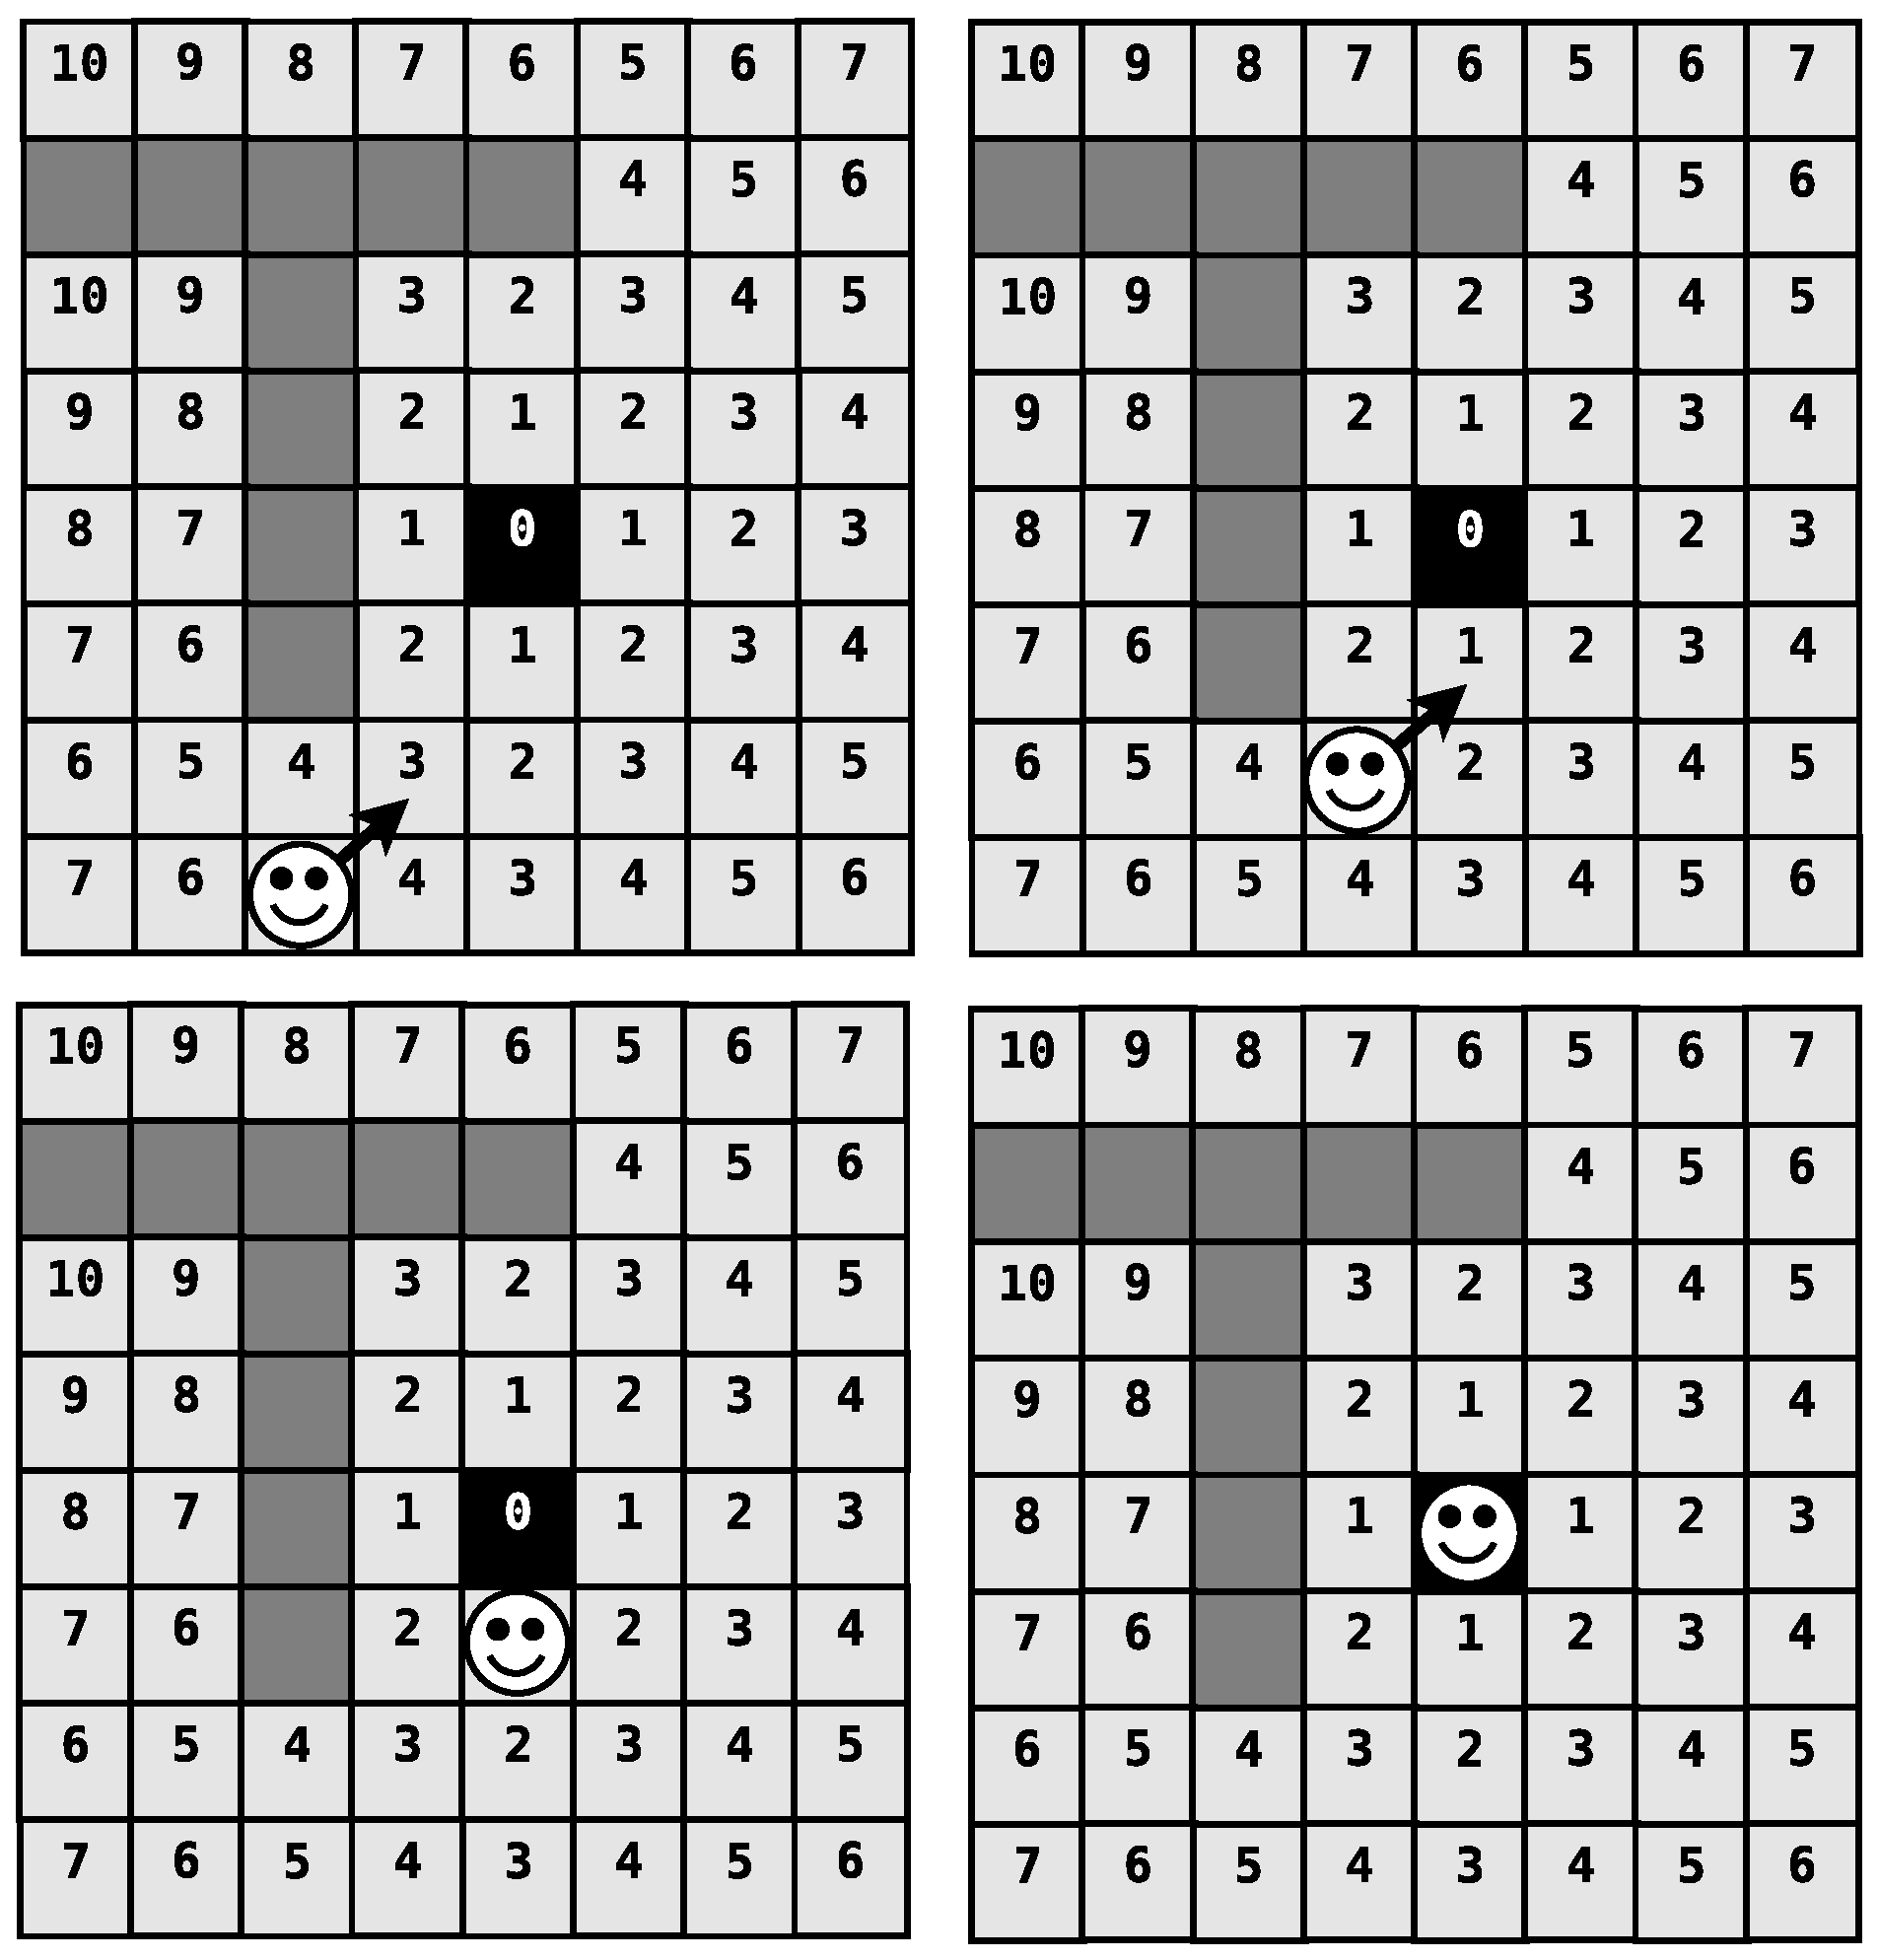
\includegraphics[height=0.65\textwidth]{simulationsumgebung/fleeing}
\caption{Fluchtwegermittlung}
\label{fig:fleeing}
\end{figure}

Der Algorithmus für die Fluchtwegbestimmung wird auf Grund der hohen Komplexität an dieser Stelle nicht komplett vorgestellt. Da zum Beispiel die Verfügbarkeit von Notausgängen oder Ausnahmebehandlungen berücksichtigt werden müssen. Das Prinzip verdeutlicht Algorithmus \ref{alg:fleeing}. Bei dem die Person in der lokalen Umgebung nach dem Patch mit der geringsten Zahl bzw. der geringsten Dämpfung des Signals eines Notausgangs sucht. 

\floatname{algorithm}{Algorithmus} 
\begin{algorithm}
\caption{person-move-to-exit}
\label{alg:fleeing}
\begin{algorithmic} 
\STATE nb $\leftarrow$ -1
\STATE min-noise $\leftarrow$ $\infty$
\STATE ask neighbors [\hfill\emph{; iterate all 8 neighbors}
\IF{$min$-$noise > signal$-$noise$}
\STATE min-noise $\leftarrow$ signal-noise\hfill\emph{; define best signal and direction}
\STATE nb $\leftarrow$ self
\ENDIF 
\STATE ]
\STATE face nb
\STATE forward 1
\end{algorithmic}
\end{algorithm}




Die Information über die Verfügbarkeit eines Notausganges wird von diesem durch das Kommunikationsnetzwerk der Personen gebroadcastet. Eine Beschreibung dazu ist dem Abschnitt \ref{sec:notausgaenge_kommunikation} Kommunikationsmodell der Notausgänge zu entnehmen.

\subsection{Kommunikationsmodell}
\label{sec:kommunikationsmodell}
%Kommunikationsmodell: Als Kommunikationsmodell können beliebige Modelle der Vorlesung implementiert werden. Dabei sollte insbesondere auf die dynamische Netzwerktopologie geach-tet werden. 

Für die Warnung anderer Personen wird das Kommunikationsmodell \emph{Basic Flooding} aus der Vorlesung implementiert. Die identifizierende Meldung lautet hier \verb|event-detected| und die beiden Zustände für das \emph{Basic Flooding} werden mit \verb|EVENT_DETECTED| und \verb|FLEEING| ausgedrückt. 

Algorithmus \ref{alg:event_detected} zeigt, zur besseren Einordnung, die Einbettung des Kommunkationsprotokolls in den Lebenszyklus der Person. Es sei darauf hingewiesen, dass auf eine spontane Zustandsänderung einer Person, wie es in dem \emph{Basic Flooding}-Protokoll angegeben ist, verzichtet wird. Die Detektion einer Gefahrensituation präzisiert diesen Zustandsübergang in diesem Fall präziser.

%\floatname{algorithm}{Protokoll} 
\begin{algorithm}
\caption{Warnung vor Gefahrensituationen}
\label{alg:event_detected}
\begin{algorithmic} 
\STATE \textit{State Trans. Sys.:} $\langle\{$INIT, EVENT{\_}DETECTED, FLEEING, RESCUED$\}, \{$INIT, DEAD$\}, \{$INIT, EVENT{\_}DETECTED, DEAD$\}, \{$INIT, EVENT{\_}DETECTED, FLEEING, DEAD$\}, \{$FLEEING, EVENT{\_}DETECTED$\}\rangle$
\STATE \textit{Initialization:} All notes in state INIT
\STATE \textit{Restrictions:} Reliable communication; connected, bidirected communication graph $G = (V,E)$, neighborhoodfunction nbr: $V \rightarrow 2^{V}$
\STATE \textit{Local data:}

\STATE $ $
\STATE \textbf{INIT}
\STATE Receiving(\textit{event{\_}detected})
\WHILE{\textit{not event{\_}detected}}
\STATE random-walk
\STATE create-graph($G$)\hfill\emph{; generate complete new graph}
\ENDWHILE
\STATE become EVENT{\_}DETECTED
\IF{touching-gas}
\STATE become DEAD
\ENDIF

\STATE $ $
\STATE \textbf{EVENT{\_}DETECTED}
\STATE broadcast(\textit{event{\_}detected})\hfill\emph{; broadcast event detection to linked neighbors}
\STATE become FLEEING
\IF{touching-gas}
\STATE become DEAD
\ENDIF

\STATE $ $
\STATE \textbf{FLEEING}
\IF{msg = event-detected}
\STATE broadcast(\textit{event{\_}detected})\hfill\emph{; forwarding event detection msg to linked neighbors}
\ENDIF
\WHILE{\textit{not person-reach-exit}}
\STATE person-move-to-exit\hfill\emph{; using orientation-algorithm}
\STATE create-graph($G$)\hfill\emph{; generate complete new graph}
\IF{event{\_}detected}
\STATE become EVENT{\_}DETECTED
\ENDIF
\IF{touching-gas}
\STATE become DEAD
\ENDIF
\ENDWHILE
\STATE become RESCUED

\STATE $ $
\STATE \textbf{RESCUED}
\STATE create-graph($G$)\hfill\emph{; generate complete new graph without note}

\STATE $ $
\STATE \textbf{DEAD}
\STATE create-graph($G$)\hfill\emph{; generate complete new graph without note}

\end{algorithmic}
\end{algorithm}

Das Fluten mit Meldungen ist jedoch ohne eine sinnvolle Netzwerktopologie nicht möglich. Mit dem Parameter \verb|graph-type| hat der Nutzer die Möglichkeit den Graph-Typen des Kommunikationsnetzwerks anzupassen. 

Allerdings wird in den meisten Fällen keine statische Knoten-Positionierung vorliegen\footnote{Eine statische Knoten-Positionierung wird mit $walk$-$probability = 0$ erzielt.}. Es wird daher nach jedem Tick der gesamte Kommunikationsgraph neu aufgebaut. Auf eine Ausnahmebehandlung für Personen ohne Positionsänderung wird verzichtet.

Zur visuellen Unterstützung erhalten Personen im Zustand \verb|EVENT_DETECTED| das Label \glqq !{\grqq}. Der initiale Broadcast zur Warnung anderer Personen wird mit orange gefärbten Kanten und der Zustand \verb|FLEEING| mit dem Label \glqq *{\grqq} ausgedrückt.



%%%%%%%%%%%%%%%%%%%%%%%%%%%%%%%%%%%%%%%%%%%%%%%%%%%%%%%%%%%%%%%%%%%%%%%%%%%%%%%%%
%%%%%%%%%%%%%%%%%%%%%%%%%%%%%%%%%%%%%%%%%%%%%%%%%%%%%%%%%%%%%%%%%%%%%%%%%%%%%%%%%

\section{Notausgänge}
\label{sec:notausgaenge}
%Notausgänge: Notausgänge sollen als statische Sensorknoten modelliert werden, die ihre Po-sition sowie Information zu ihrer Passierbarkeit im Netz verteilen. Die Positionen dieser sog. anchor nodes sollen zur Positionierung der mobilen Sensorknoten verwendet werden (Algorithmik). Während einer Simulation sollte der Ausfall einzelner Notausgänge simuliert werden.

Notausgänge sind statische Agenten, für die eine eigene \emph{breed} analog zu den Personen angelegt wurde. Die Notausgänge verfügen über einen Lebenszyklus und ein Kommunikationsmodell zur Übermittlung ihrer Zustandsinformationen an nahe Personen. 

%Lifecycle
\subsection{Lebenszyklus}

% INIT, NEGOTIABLE
% INIT, NEGOTIABLE, BLOCKED

Der Lebenszyklus eines Notausgangs ist in drei Zustände unterteilt. Im Zustand \verb|INIT| befinden sich alle Notausgänge nach der Platzierung auf der Welt. Während des Zustandsübergangs zu \verb|NEGOTIABLE| wird die Logik für den gewählten Orientierungsalgorithmus ausgeführt. In der Regel wird die Welt mit Signalinformationen ausgehend von jedem Notausgang geflutet. Der Algorithmus wird in Kapitel \ref{cha:algorithmik} vorgestellt. Die Ausführung dauert entsprechend der (Patch-)Auflösung lange.

Ist ein Notausgang im Zustand \verb|NEGOTIABLE|, bestehen zwei Möglichkeiten in den Zustand \verb|BLOCKED| zu gelangen. Temporär blockiert ist ein Notausgang, wenn zu viele Personen gleichzeitig versuchen das Gebäude zu verlassen. Der Parameter \verb|exit-limit| definiert die Obergrenze. Nach einem Tick wird der Notausgang wieder zurückgesetzt. Erreicht das Giftgas bzw. die Gefahrensituation einen Notausgang, so wird dieser permanent in den Zustand \verb|BLOCKED| über.

\begin{figure}[!ht]
\centering
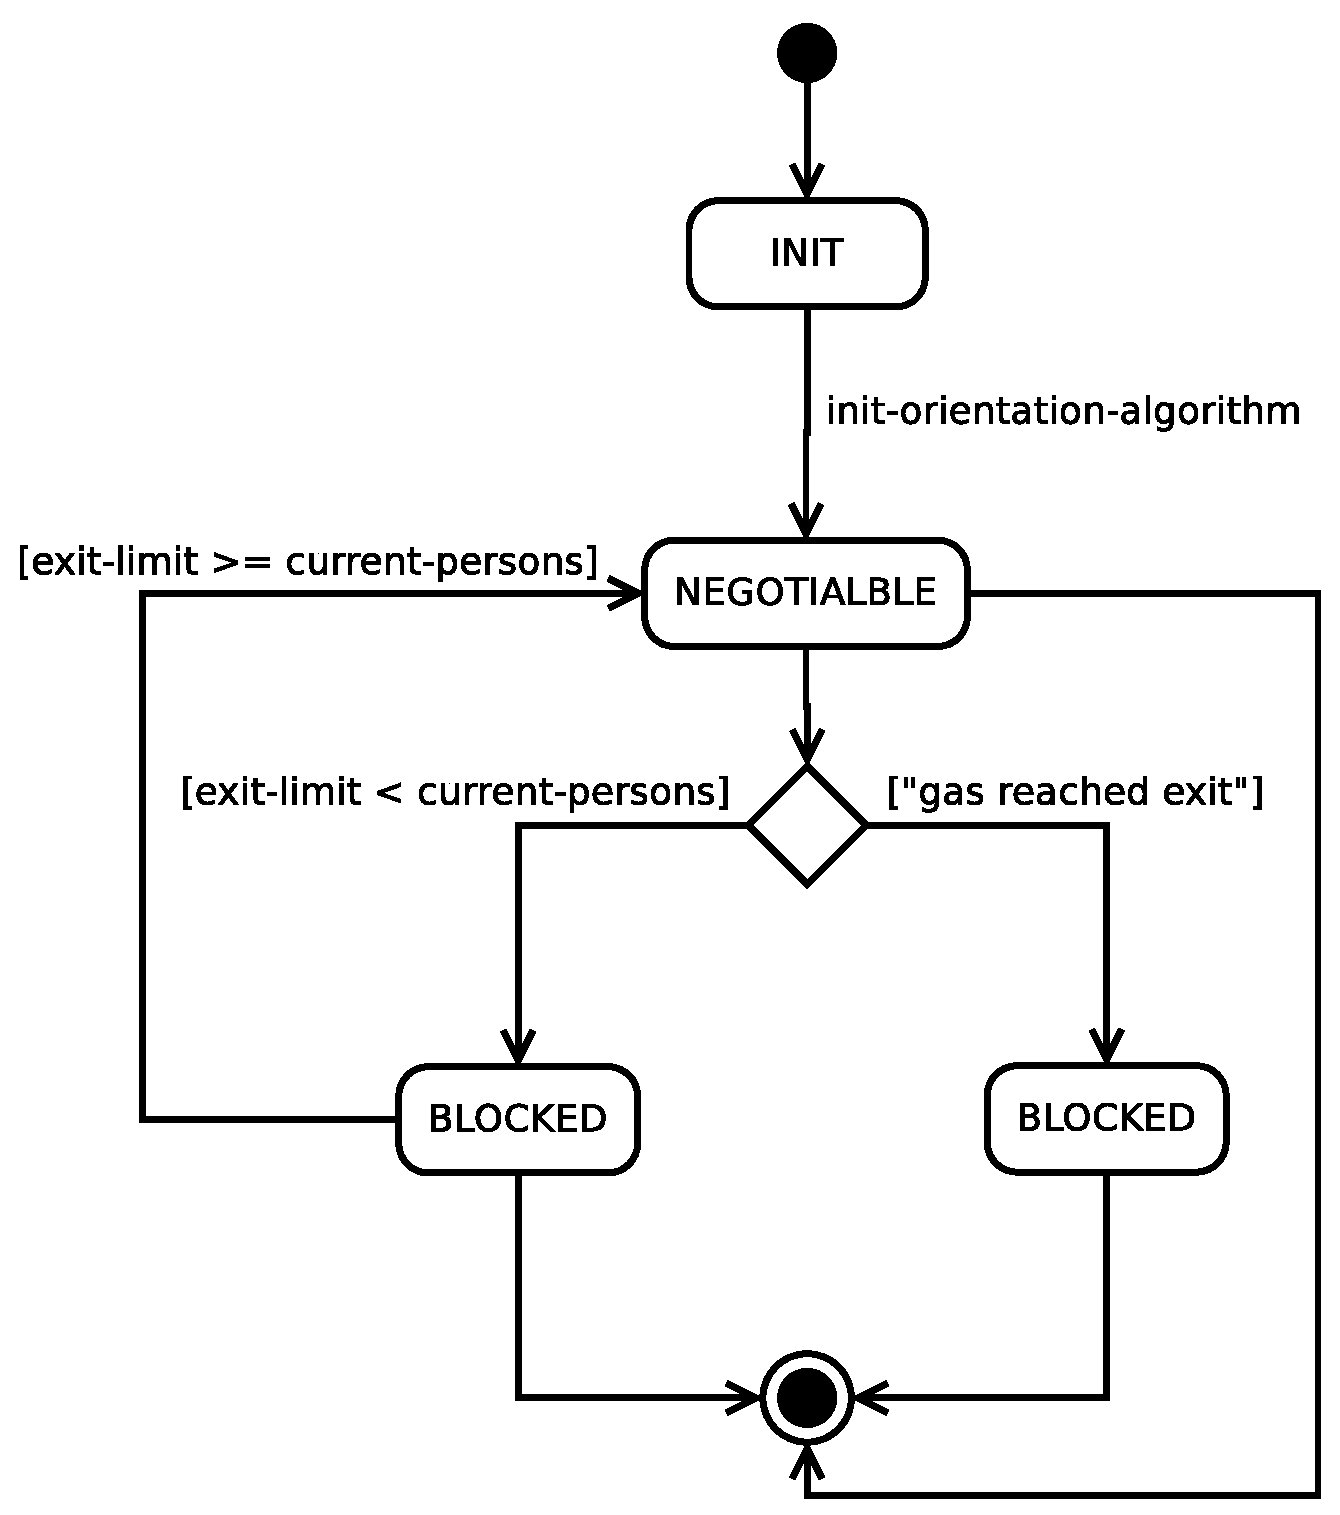
\includegraphics[height=0.6\textwidth]{simulationsumgebung/exit.eps}
\caption{Zustandsdiagramm der Notausgänge}
\label{fig:exit}
\end{figure}

%\begin{algorithm}
%\caption{Patch-Flooding (Zellulärer Automat)}
%\begin{algorithmic} 
%\STATE \textit{State Trans. Sys.:} $\langle\{$NONE$\},\{$NONE, SPREADING, IDLE, DONE$\}\rangle$
%\STATE \textit{Initialization:} All patches in state NONE
%\STATE \textit{Restrictions:} orientation-algorithm = $"$Cellular automaton$"$
%\STATE \textit{Global data:} exit-signal-strength $\in \mathbb{N}_{\geq0}$
%\STATE \textit{Local data:} 
%\STATE Set \textit{exits} of exits in range
%\STATE Set \textit{signal-noises} of exit signals
%
%\STATE $ $
%\STATE \textbf{NONE}
%\STATE \textit{Spontaneously}
%\STATE exits $\leftarrow$ myself\hfill\emph{;exit on this patch}
%\STATE signal-noises $\leftarrow$ 0
%\STATE become SPREADING
%
%
%\STATE $ $
%\STATE \textbf{SPREADING}
%\STATE parent-exit $\leftarrow$ exit
%\STATE signal-noise-here $\leftarrow$ signal-noise + 1
%\FOR{? one-of neighbors}
%\IF{[patch-state] of ? = NONE}
%\STATE exits $\leftarrow$ parent-exit
%\STATE signal-noises $\leftarrow$ signal-noise-here
%\ENDIF
%\ENDFOR
%\STATE become IDLE
%
%
%\STATE $ $
%\STATE \textbf{IDLE}
%
%\STATE become DONE
%
%\STATE $ $
%\STATE \textbf{DONE}
%
%\end{algorithmic}
%\end{algorithm}

\subsection{Kommunikationsmodell}
\label{sec:notausgaenge_kommunikation}

Die Notausgänge befinden sich im gleichen Kommunikationsnetzwerk, wie die Personen. Eine Unterscheidung zu anderen Netzwerken bzw. Links wird über Typ-Definitionen und visuell über den Shape durchgeführt.

\floatname{algorithm}{Algorithmus} 
\begin{algorithm}
\caption{Passierbarkeitsmeldungen der Notausgänge}
\label{alg:exit_status}
\begin{algorithmic} 
\STATE \textit{State Trans. Sys.:} $\langle\{$INIT, NEGOTIABLE, BLOCKED$\}, \{$NEGOTIABLE, BLOCKED$\}, \{$BLOCKED, NEGOTIABLE$\}\rangle$
\STATE \textit{Initialization:} All notes in state INIT
\STATE \textit{Restrictions:} Reliable communication; connected, bidirected communication graph $G = (V,E)$, neighborhoodfunction nbr: $V \rightarrow 2^{V}$
\STATE \textit{Local data: current-persons, exit-limit}

\STATE $ $
\STATE \textbf{INIT}
\STATE ...\hfill\emph{; init-orientation-algorithm}
\STATE become NEGOTIABLE

\STATE $ $
\STATE \textbf{NEGOTIABLE}
\STATE negotiable $\leftarrow$ true
\WHILE{$negotiable$}
\STATE broadcast(\textit{exit-negotiable})\hfill\emph{; continious broadcast}
\IF{$current$-$persons > exit$-$limit$}
\STATE negotiable $\leftarrow$ false
\ENDIF
\IF{$gas$-$reached$-$exit$}
\STATE negotiable $\leftarrow$ false
\ENDIF
\ENDWHILE
\STATE become BLOCKED


\STATE $ $
\STATE \textbf{BLOCKED}
\STATE negotiable $\leftarrow$ false
\WHILE{$not negotiable$}
\STATE broadcast(\textit{exit-blocked})\hfill\emph{; continious broadcast}
\IF{$current$-$persons <= exit$-$limit$}
\STATE negotiable $\leftarrow$ true
\ENDIF
\ENDWHILE
\STATE become NEGOTIABLE

\end{algorithmic}
\end{algorithm}

Für die Verbreitung der Passierbarkeit wird das \emph{Basic Flooding} implementiert. Algorithmus \ref{alg:exit_status} zeigt das eingebettete Protokoll innerhalb des Lebenszyklus von Notausgängen. 

Die Notausgänge broadcasten bei Statuswechsel eine positive oder negative Passierbarkeitsmeldung und ihren Identifier im Netzwerk. Personen in Reichweite empfangen die Meldung \verb|exit-blocked| oder \verb|exit-negotiable|, speichern die Information lokal in einem binären Array ab und broadcasten die Meldung an die benachbarten Personen. Bei n = 3 Notausgängen verfügt jede Person über ein n-äres Array mit Nullen oder Einsen. Null steht für blockiert, Eins für passierbar.





%%%%%%%%%%%%%%%%%%%%%%%%%%%%%%%%%%%%%%%%%%%%%%%%%%%%%%%%%%%%%%%%%%%%%%%%%%%%%%%%%
%%%%%%%%%%%%%%%%%%%%%%%%%%%%%%%%%%%%%%%%%%%%%%%%%%%%%%%%%%%%%%%%%%%%%%%%%%%%%%%%%

\section{Gefahrensituationen}
\label{sec:gefahrensituationen}
%Gefahrenevents: Gefahrenevents erscheinen an zufälligen Orten im Grundriss. Ihr Erscheinen sollte zur vollständigen Evakuierung des Areals führen.

Eine Gefahrensituation liegt vor, wenn nur ein Gefahrenevent aktiviert wurde. Die Gefahrenevents werden als \emph{breed} modelliert. 

%Lifecyle
\subsection{Lebenszyklus}

% INIT, COUNTDOWN, GASSING, DONE

Die Zustandsübergänge von Gefahrenevents verlaufen sequentiell. Alle Events beginnen nach der Platzierung im Zustand \verb|INIT| und enden im Zustand \verb|DONE|. Abbildung \ref{fig:event} zeigt ebenfalls die beiden weiteren Zustände \verb|COUNTDOWN| und \verb|GASSING|.

\begin{figure}[!ht]
\centering
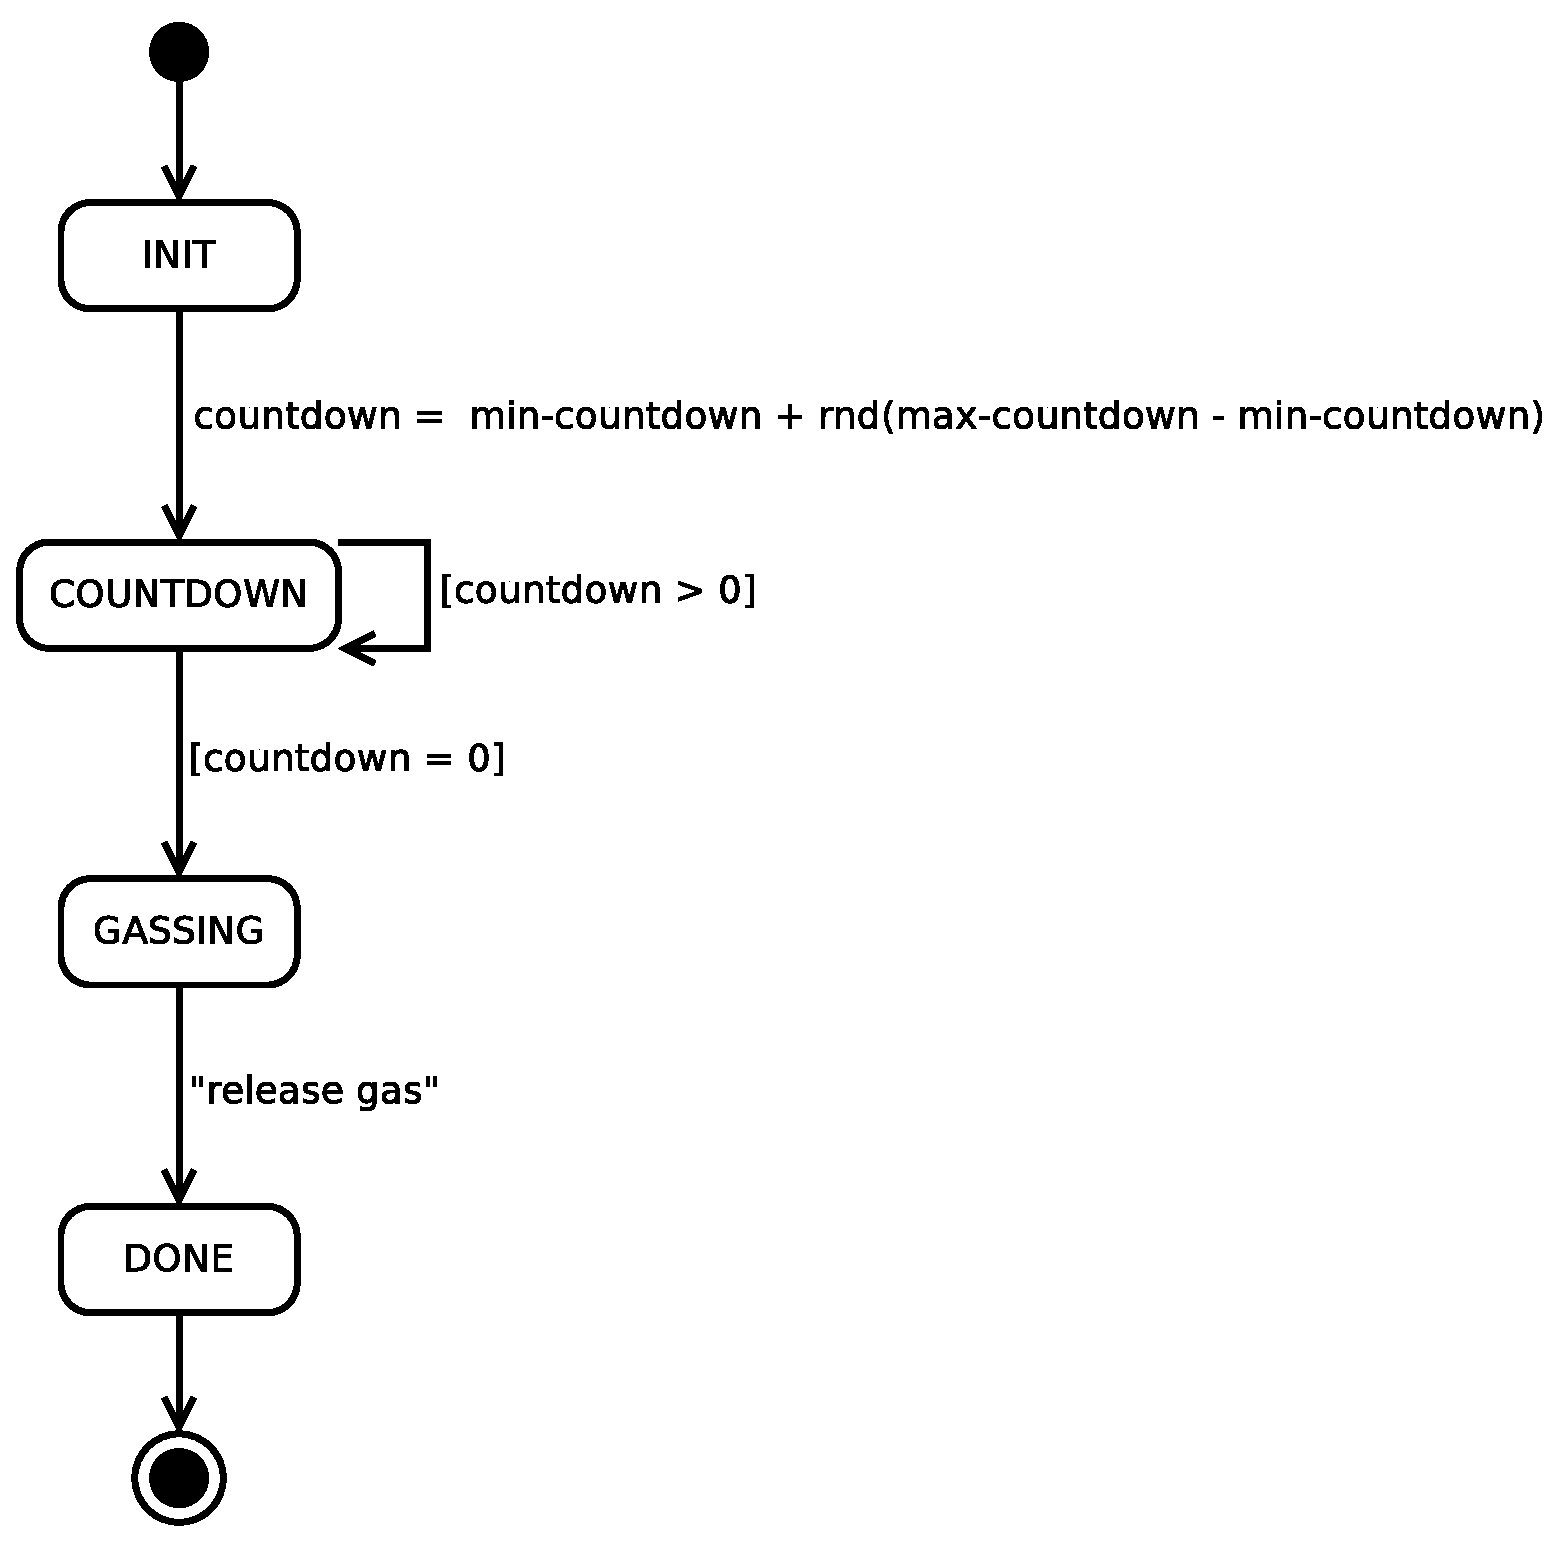
\includegraphics[height=0.5\textwidth]{simulationsumgebung/event.eps}
\caption{Zustandsdiagramm der Gefahrenevents}
\label{fig:event}
\end{figure}

Mit dem Start der Simulation gehen alle Events in den Zustand \verb|COUNTDOWN| über, in der lokal vorgehaltene zufällige Countdown pro Tick herunter gezählt wird. Steht der Countdown bei Null, geht das Gefahrenevent in den Zustand \verb|GASSING| über.

In diesem Zustand wird die Freisetzung des Gases initiiert. Die Ausbreitung des Gases ähnelt dem Fluten mit Signal-Informationen auf Kapitel \ref{cha:algorithmik}. 
%Der Algorithmus \ref{alg:event} liefert detailierte Informationen zur Bestimmung des zufälligen Countdowns und der Gasfreisetzung, die im folgenden Abschnitt zu den Patches noch einmal angesprochen wird.

%\begin{algorithm}
%\caption{Gefahrensituation}
%\label{alg:event}
%\begin{algorithmic} 
%\STATE \textit{State Trans. Sys.:} $\langle\{$INIT, COUNTDOWN, GASSING, DONE$\}\rangle$
%\STATE \textit{Initialization:} All notes in state INIT
%\STATE \textit{Restrictions:} All patches in state $\{$NONE, DONE$\}$
%\STATE \textit{Local data:} countdown $\in \mathbb{N}_{\geq0}$ 
%\STATE $ $
%\STATE \textbf{INIT}
%\STATE \textit{Spontaneously}
%
%\STATE countdown $\leftarrow$ minCountdown + (random (maxCountdown - minCountdown))
%\STATE become COUNTDOWN
%
%
%\STATE $ $
%\STATE \textbf{COUNTDOWN}
%\STATE countdown $\leftarrow$ countdown - 1
%\IF{$countdown = 0$}
%\STATE become GASSING
%\ENDIF
%
%\STATE $ $
%\STATE \textbf{GASSING}
%\STATE ask patch-here $[$ patch-state $\leftarrow$ EVENT $]$ 
%\STATE become DONE
%
%\STATE $ $
%\STATE \textbf{DONE}
%
%\end{algorithmic}
%\end{algorithm}

%%%%%%%%%%%%%%%%%%%%%%%%%%%%%%%%%%%%%%%%%%%%%%%%%%%%%%%%%%%%%%%%%%%%%%%%%%%%%%%%%
%%%%%%%%%%%%%%%%%%%%%%%%%%%%%%%%%%%%%%%%%%%%%%%%%%%%%%%%%%%%%%%%%%%%%%%%%%%%%%%%%

\section{Patches}
\label{sec:patches}

- Initialisierung der Patches setup-patches
 - Zustandsfestlegung für alle Patches 
  - white -> NONE
  - black -> WALL
  - rest -> WALL
 - Initialisierung der lokalen Daten \verb|signal-noise| abhängig vom Zustand: leerer Raum -> -1, Wand -> sehr hohe Dämpfung \ref{sec:gui_exit} 


%Lifecyle
\subsection{Implizite Zustände}
\label{sec:patch_states}
% NONE, WALL, SPREADING, IDLE, DONE, EVENT, EVENT-DONE

% Kategorie: Grundriss
% NONE
% WALL

% Kategorie: Zellulärer Automat
% NONE
% NONE, SPREADING, IDLE, DONE

% Kategorie: Gefahrensituation
% NONE, EVENT
% NONE, EVENT, EVENT_DONE
% DONE, EVENT
% DONE, EVENT, EVENT_DONE

\begin{figure}[!ht]
\centering
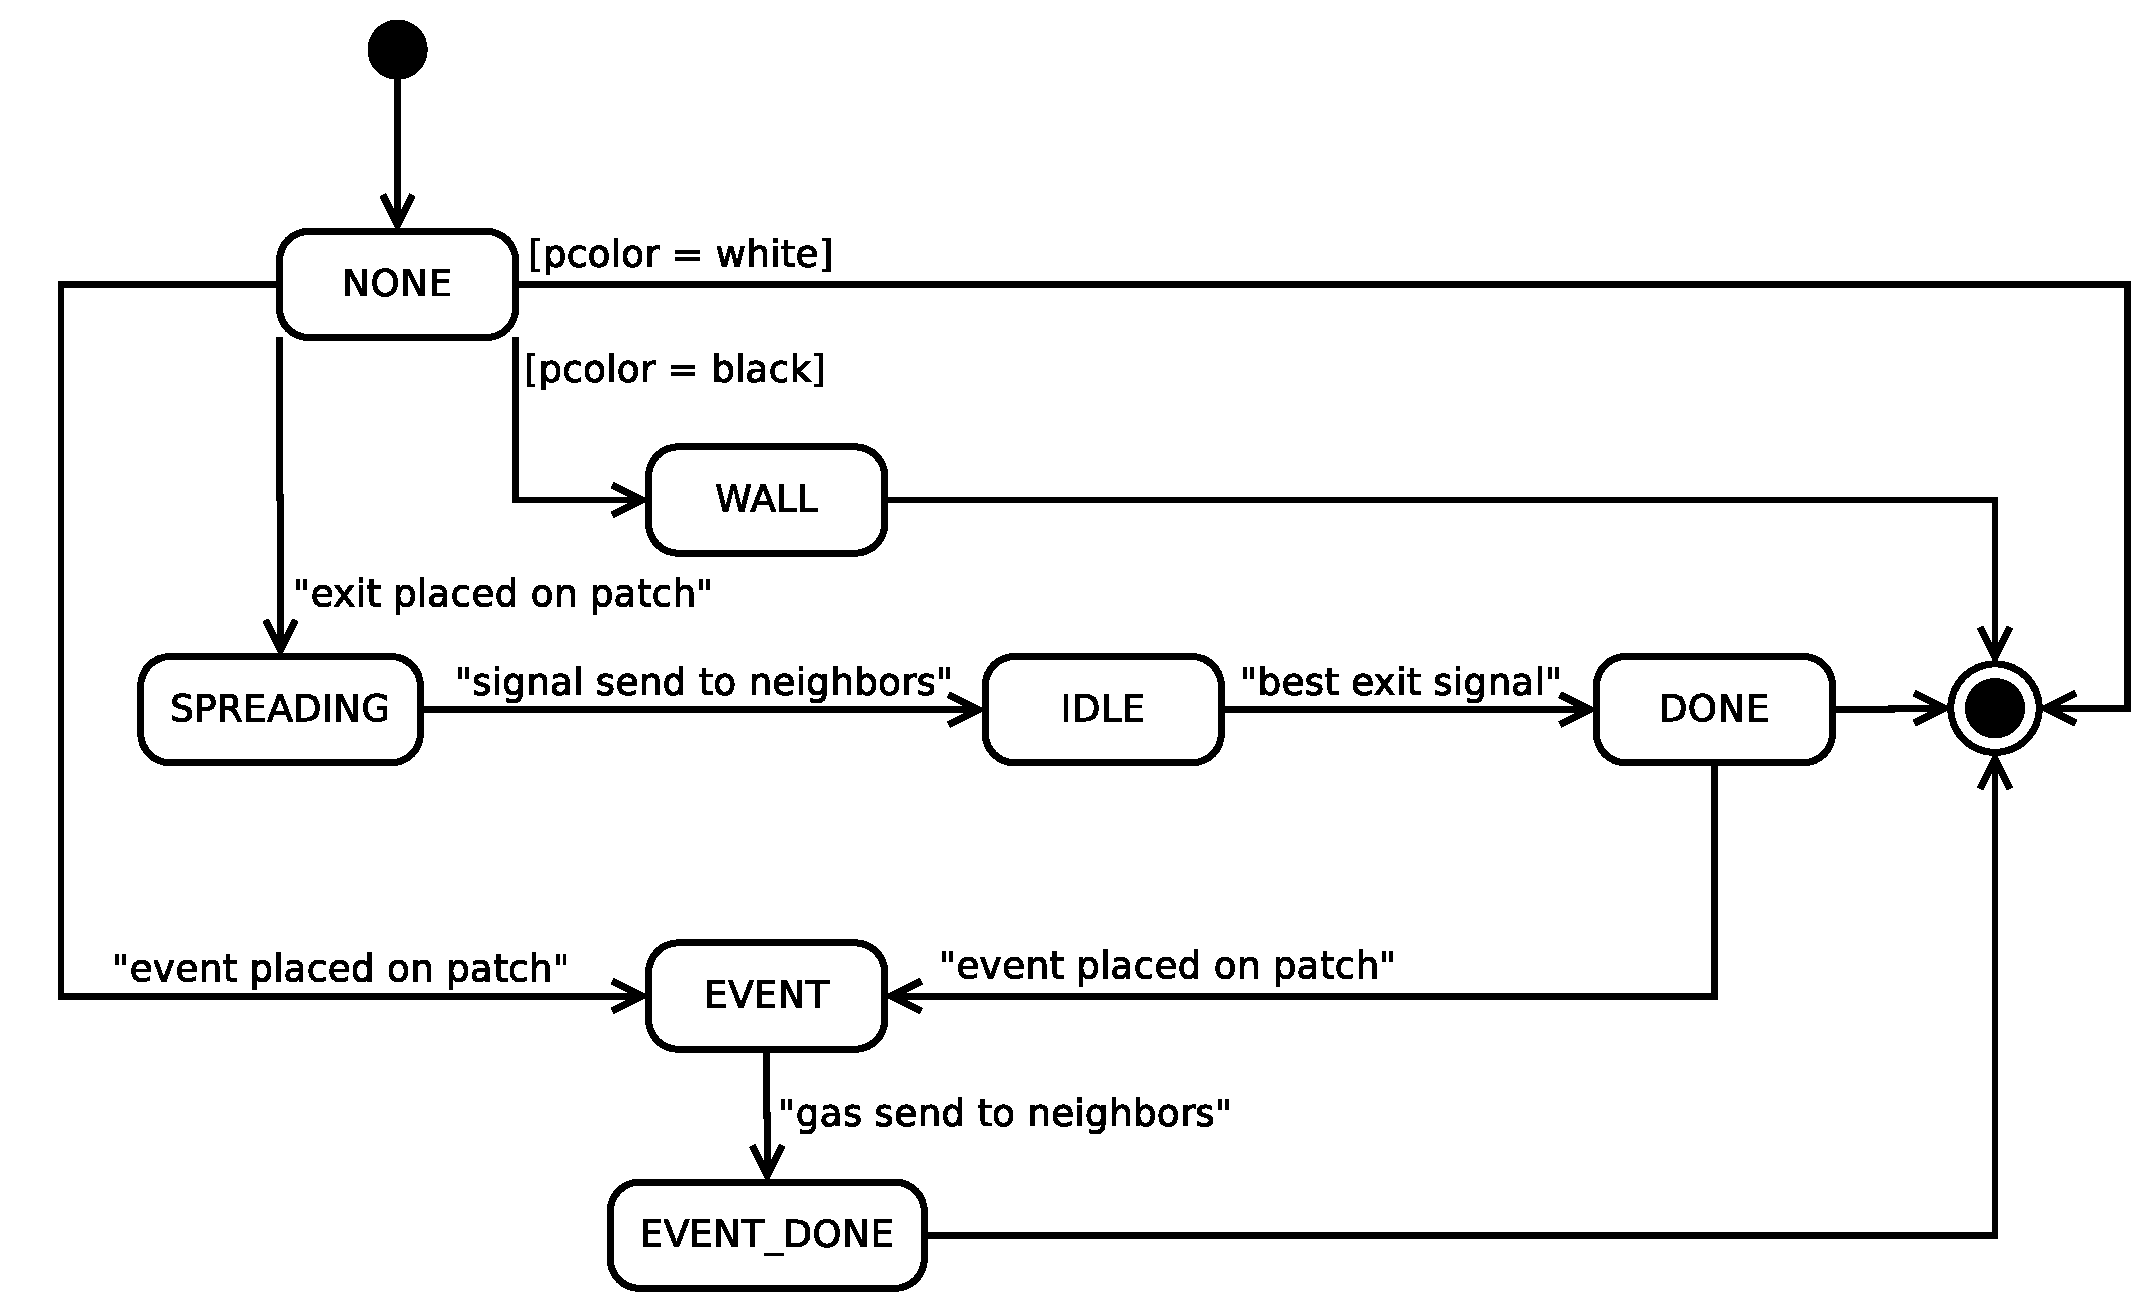
\includegraphics[height=0.6\textwidth]{simulationsumgebung/patch.eps}
\caption{Zustandsdiagramm der Patches}
\label{fig:patch}
\end{figure}

%%%%%%%%%%%%%%%%%%%%%%%%%%%%%%%%%%%%%%%%%%%%%%%%%%%%%%%%%%%%%%%%%%%%%%%%%%%%%%%%%
%%%%%%%%%%%%%%%%%%%%%%%%%%%%%%%%%%%%%%%%%%%%%%%%%%%%%%%%%%%%%%%%%%%%%%%%%%%%%%%%%

\section{Ressourcen der Simulationsumgebung}
\label{sec:ressourcen}

Die Simulationsumgebung wird über die Datei \verb|Evakuierung.nlogo| gestartet. Der Programmcode ist nach Funktion und \emph{Breed}-Klasse unterteilt.

\paragraph{Gefahrensituationen} 

\begin{verbatim}
event.nls
event-gassing.nls
\end{verbatim}

Die Quellcode-Datei \verb|event.nls| beinhaltet den Lebenszyklus der Gefahrenevents und deren Zustandsübergangsprotokoll. Mittels \verb|event-gassing.nls| wird die Ausbreitung des Giftgases implementiert, die größtenteils den Patch-Lebenszyklus manipuliert.

\paragraph{Lokalisierung}

\begin{verbatim}
locate.nls
\end{verbatim}

In dieser Datei wird der Algorithmus zur Lokalisierung aus dem Paper \cite{Jonathan.2004} implementiert.

\paragraph{Notausgänge}

\begin{verbatim}
exit.nls
exit-cellular-automaton.nls
exit-gsn.nls
\end{verbatim}

Die Quellcode-Datei \verb|event.nls| steuert den Setup und den Lebenszyklus der Notausgänge. Mittels \verb|exit-cellular-automaton.nls| wird der Orientierungsalgorithmus auf Basis des zellulären Automats realisiert. Letztlich definiert die Datei \verb|exit-gsn.nls| das Kommunikationsmodell zur Übermittlung der Statusinformationen.

\paragraph{Personen}

\begin{verbatim}
person.nls
person-gsn.nls
person-linking.nls
\end{verbatim}

\verb|person.nls| regelt den Setup der Personen und deren Lebenszyklus. \verb|person-gsn.nls| umfasst den Quellcode für die Kommunikation zwischen Personen und mit der Datei \verb|person-linking.nls| wird der Graph zwischen Personen erstellt.

\paragraph{Simulationswelt}

\begin{verbatim}
patch.nls
\end{verbatim}

Hier wird der Quellcode für den Lebenszyklus der \emph{Patches} definiert.
\chapter{Algorithmik}
\label{cha:algorithmik}
%Damit die mobilen Geräten den Nutzern Hinweise zum nächsten Notausgang geben können, müssen sie ihre eigene Position kennen. Daher soll ein dezentraler Lokalisierungsalgorithmus implementiert werden (siehe [2]). Beispielweise kann der minimale Nachrichten Hop-Count zu einem Notausgang im Zusammenhang mit der maximalen Kommunikationsreichweite zur Ap-proximation der Distanz des Knotens zum Ausgang dienen (siehe [1], gradient algorithm). Meh-rere (>=3) dieser Distanzen können wiederum zur Positionierung verwendet werden (Stichwort: Lateration. Siehe multilateration algorithm in [1] oder Bogenschnitt). In der Visualisierung sollte die Qualität der Positionierung erkennbar sein, d.h. es sollte zusätzlich zur wahren Position des Sensorknotens die errechnete Position erkennbar sein. 

\section{Multilateration Lokalisierung}
\label{sec:gradient_localization}

Der Algorithmus startet beim Setup der Simulation mit der Bestimmung der Hop Counts von allen Personen zu allen Ausgängen. Der \emph{Hop Count} repräsentiert im Netzwerk die Anzahl der Sprünge, die benötigt wird, um einen Knoten zu erreichen. Sei beispielsweise ein Notausgang mit einer Person verbunden, so hat sie einen Hop Count von 1 vom Notausgang aus. Ist diese Person mit einer anderen Person verbunden, die wiederum \emph{nicht} mit dem Notausgang verbunden ist, so hat sie einen Hop Count von 2.

\paragraph{Theorie} 

Nachdem die geschätzten Distanzen zu den Orientierungspunkten (Notausgängen) zu jeder Person berechnet sind, ist es möglich, eine Abschätzung der Position dieser Person zu machen. Dafür benötigt man mindestens 3 Punkte, es werden jedoch wesentlich mehr Punkte benötigt, um eine bessere Approximation zu der echten Position zu erreichen (vergleiche \cite{Jonathan.2004} ab Seite 217, Kapitel Analysis). 

\begin{equation} \label{eq:dist}
d_{ij} = \sqrt{(x_i - x_j)^2 + (y_i - y_j)^2}
\end{equation}

In der Formel \ref{eq:dist} bestimmen wir die Formel, die die Distanz zwischen einem Orientierungspunkt j und einem beliebigen Punkt i beschreibt. Das benutzen wir, um die tatsächliche Distanz zu der Person mit der Distanz zum geschätzten Punkt zu vergleichen.

\begin{equation} \label{eq:error}
E_j = \sum_{i=1}^{n} (d_{ji} - \hat d_{ji})^2
\end{equation}

In der Formel \ref{eq:error} bestimmt die Summe des quadrierten Fehler, d.h. die Fehleinschätzung unserer geschätzten Distanz zu der tatsächlichen Distanz. Dabei ist \( d \) die tatsächliche Position und \( \hat d \) die geschätzte Position. Nun ist also \( d \) die unbekannte und wir wollen diesen Fehler minimieren.

\begin{equation} \label{eq:abl}
 \frac{\partial E_j}{\partial x_i} = \sum_{i=1}^{n}(x_j - x_i) \left( 1-\frac{d_{ji}}{\hat d_{ji}} \right) \textrm{ and }  \frac{\partial E_j}{\partial y_i} = \sum_{i=1}^{n}(y_j - y_i) \left( 1-\frac{d_{ji}}{\hat d_{ji}} \right)
\end{equation}

Um den Fehler zu minimieren bilden wir die partiellen Ableitungen in \ref{eq:abl} und versuchen so, nach Methoden der Analysis, das Minimum zu bestimmen. Wir starten also mit einer geschätzten Position \( \hat d \) und verschieben langsam die Punkte um \( \alpha \) und minimieren damit den Fehler.

\paragraph{Implementierung} 

\begin{figure}[h!]
\centering
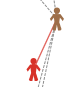
\includegraphics{algorithmik/visu}
\caption{Visualisierung der geschätzten Positionen}
 \label{visu}
\end{figure}

In der Implementierung wählen wir als Punkt \( \hat d \) den Ausgang, der dem Charakter laut hop count am nächsten steht, da jede Person die Position aller Notausgänge im Netzwerk kennt. Bei der Implementierung orientiert sich der Algorithmus an den Referenzcode der zur Verfügung gestellt wurde. Nachdem der Hop Count beim Setup für jede Person bestimmt wurde, kann der Algorithmus für jede Person ausgeführt werden. Wieviele Iterationen vorgenommen werden, ist ein einstellbarer Parameter. Nachdem eine Position für eine Person geschätzt wurde, wird sie als rote Person in die Simulationsumgebung integriert und mit der richtigen Person mit einem roten Link verbunden, wie auf der Abbildung \ref{visu} zu sehen ist.







\section{Zellul\"arer Automat}
\label{sec:cellular_automaton}

%Damit die mobilen Geräten den Nutzern Hinweise zum nächsten Notausgang geben können, müssen sie ihre eigene Position kennen. Daher soll ein dezentraler Lokalisierungsalgorithmus implementiert werden (siehe [2]). Beispielweise kann der minimale Nachrichten Hop-Count zu einem Notausgang im Zusammenhang mit der maximalen Kommunikationsreichweite zur Ap-proximation der Distanz des Knotens zum Ausgang dienen (siehe [1], gradient algorithm). Meh-rere (>=3) dieser Distanzen können wiederum zur Positionierung verwendet werden (Stichwort: Lateration. Siehe multilateration algorithm in [1] oder Bogenschnitt). In der Visualisierung sollte die Qualität der Positionierung erkennbar sein, d.h. es sollte zusätzlich zur wahren Position des Sensorknotens die errechnete Position erkennbar sein

Die mobilen Geräte bestimmen über die \emph{Multilateration Lokalisierung} die approximierte Position der Personen. Daraus wird die Entfernung zu den Notausgängen geschätzt. Im Falle einer Gefahrensituation flüchten die Personen zu dem nächst gelegenen und verfügbaren Notausgang.

Für die Orientierung während der Flucht steuert die Umgebung (Zelluläre Automaten) die Bewegung der Person.

Die zellulären Automaten dienen zur Modellierung räumlich diskreter dynamischer Systeme. In diesem Fall wird die zweidimensionale Simulationsumgebung als Zellularraum $Z$ und die Patches als Zellen $z \in Z$ betrachtet. Die Patches bilden ein orthogonales Gitter.

Für die endliche Nachbarschaft der Zellen ergibt sich:

\begin{quote}
$ N_{Moore}(z)=\left\{\begin{array}{cl} \vert Z_{Neighbor}\vert = 3, & \mbox{falls }Edge(z) = true,\\ \vert Z_{Neighbor}\vert = 5, & \mbox{falls }Border(z) = true,\\ \vert Z_{Neighbor}\vert = 8, & \mbox{sonst.} \end{array}\right. $

$ N_{Neumann}(z)=\left\{\begin{array}{cl} \vert Z_{Neighbor}\vert = 2, & \mbox{falls }Edge(z) = true,\\ \vert Z_{Neighbor}\vert = 3, & \mbox{falls }Border(z) = true,\\ \vert Z_{Neighbor}\vert = 4, & \mbox{sonst.} \end{array}\right. $
\end{quote}

Abbildung \ref{fig:neighborhood} visualisiert die beiden Nachbarschaftsbeziehungen, Moore-Nachbarschaft $ N_{Moore}(z)$ oder Von-Neumann-Nachbarschaft $ N_{Neumann}(z)$, für die drei Zelltypen. Zelle $z_{1}$ ist an der oberen Ecke des Raumes, Zelle $z_{2}$ am Rand und Zelle $z_{3}$ innerhalb des Zellularraums. 

\begin{figure}[!ht]
\centering
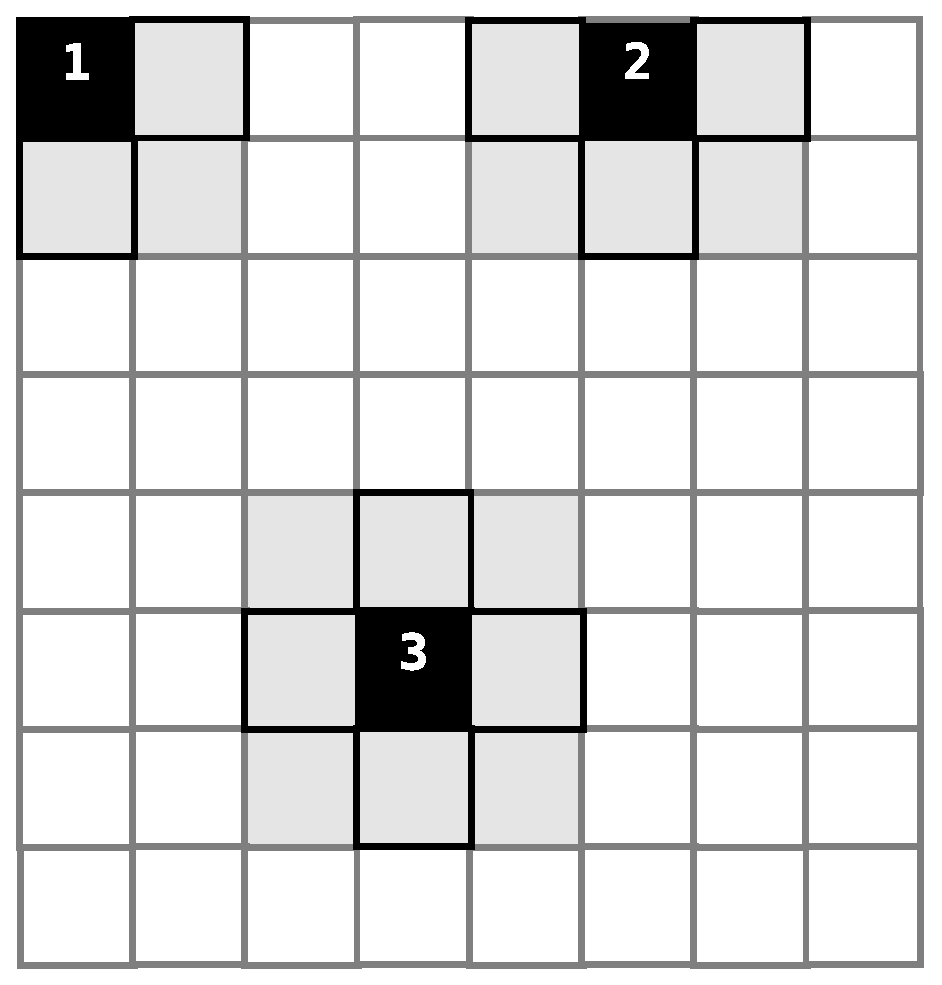
\includegraphics[height=0.3\textwidth]{algorithmik/neighborhood.eps}
\caption{Nachbarschaftsbeziehungen der Zellen}
\label{fig:neighborhood}
\end{figure}

Neben der Menge an benachbarten Zellen besitzt jede Zelle einen diskreten Zustand $q \in Q$ aus der Zustandsmenge $Q$, die bereits in Abschnitt \ref{sec:patch_states} angesprochen wurde.

\begin{quote}
$Q = \{NONE, SPREADING, IDLE, DONE\}$
\end{quote}

Zusätzlich besitzt jede Zelle lokale Zustandsübergangsregeln $\delta \colon Q^{N}\to Q$, die in Abhängigkeit mit den Zuständen und Werte aller Nachbarn zum Zeitpunkt $t$ deren neuen Zustand bestimmt. Für jeden diskreten Zeitschritt $t + 1$ werden die Zustandsübergangsregeln für alle Zellen angewendet.

Besonders ist hier, dass sowohl der Zustand einer Zelle überführt wird, als auch die Signalausbreitung der Notausgänge simuliert wird. Jede benachbarte Zelle $Z_{Neighbor} \subset Z\setminus\{z\}$ erhält den inkrementierten Signal-Dämpfungswert des Vorgängers $z \in Z$. Nachdem die dynamische Signalausbreitung abgeschlossen ist, werden die zellulären Automaten als terminiert, d.h. statisch angesehen. Zustands- und Wertänderungen sind nicht mehr möglich. Die Signalausbreitung ist beendet, sobald die maximale Dämpfung erreicht wurde.

Abbildung \ref{fig:flooding} zeigt die Zeitschritte $t_{1}$ bis $t_{9}$ bei Anwendung der Von-Neumann-Nachbarschaftsbeziehung. Die schwarze Zelle markiert die Position eines Notausgangs. Zum Zeitpunkt $t_{0}$ ist wird diese Zelle mit dem Signal-Dämpfungswert = 0 und dem Zustand \verb|SPREADING| (spontan) initialisiert.

\begin{figure}[!ht]
\centering
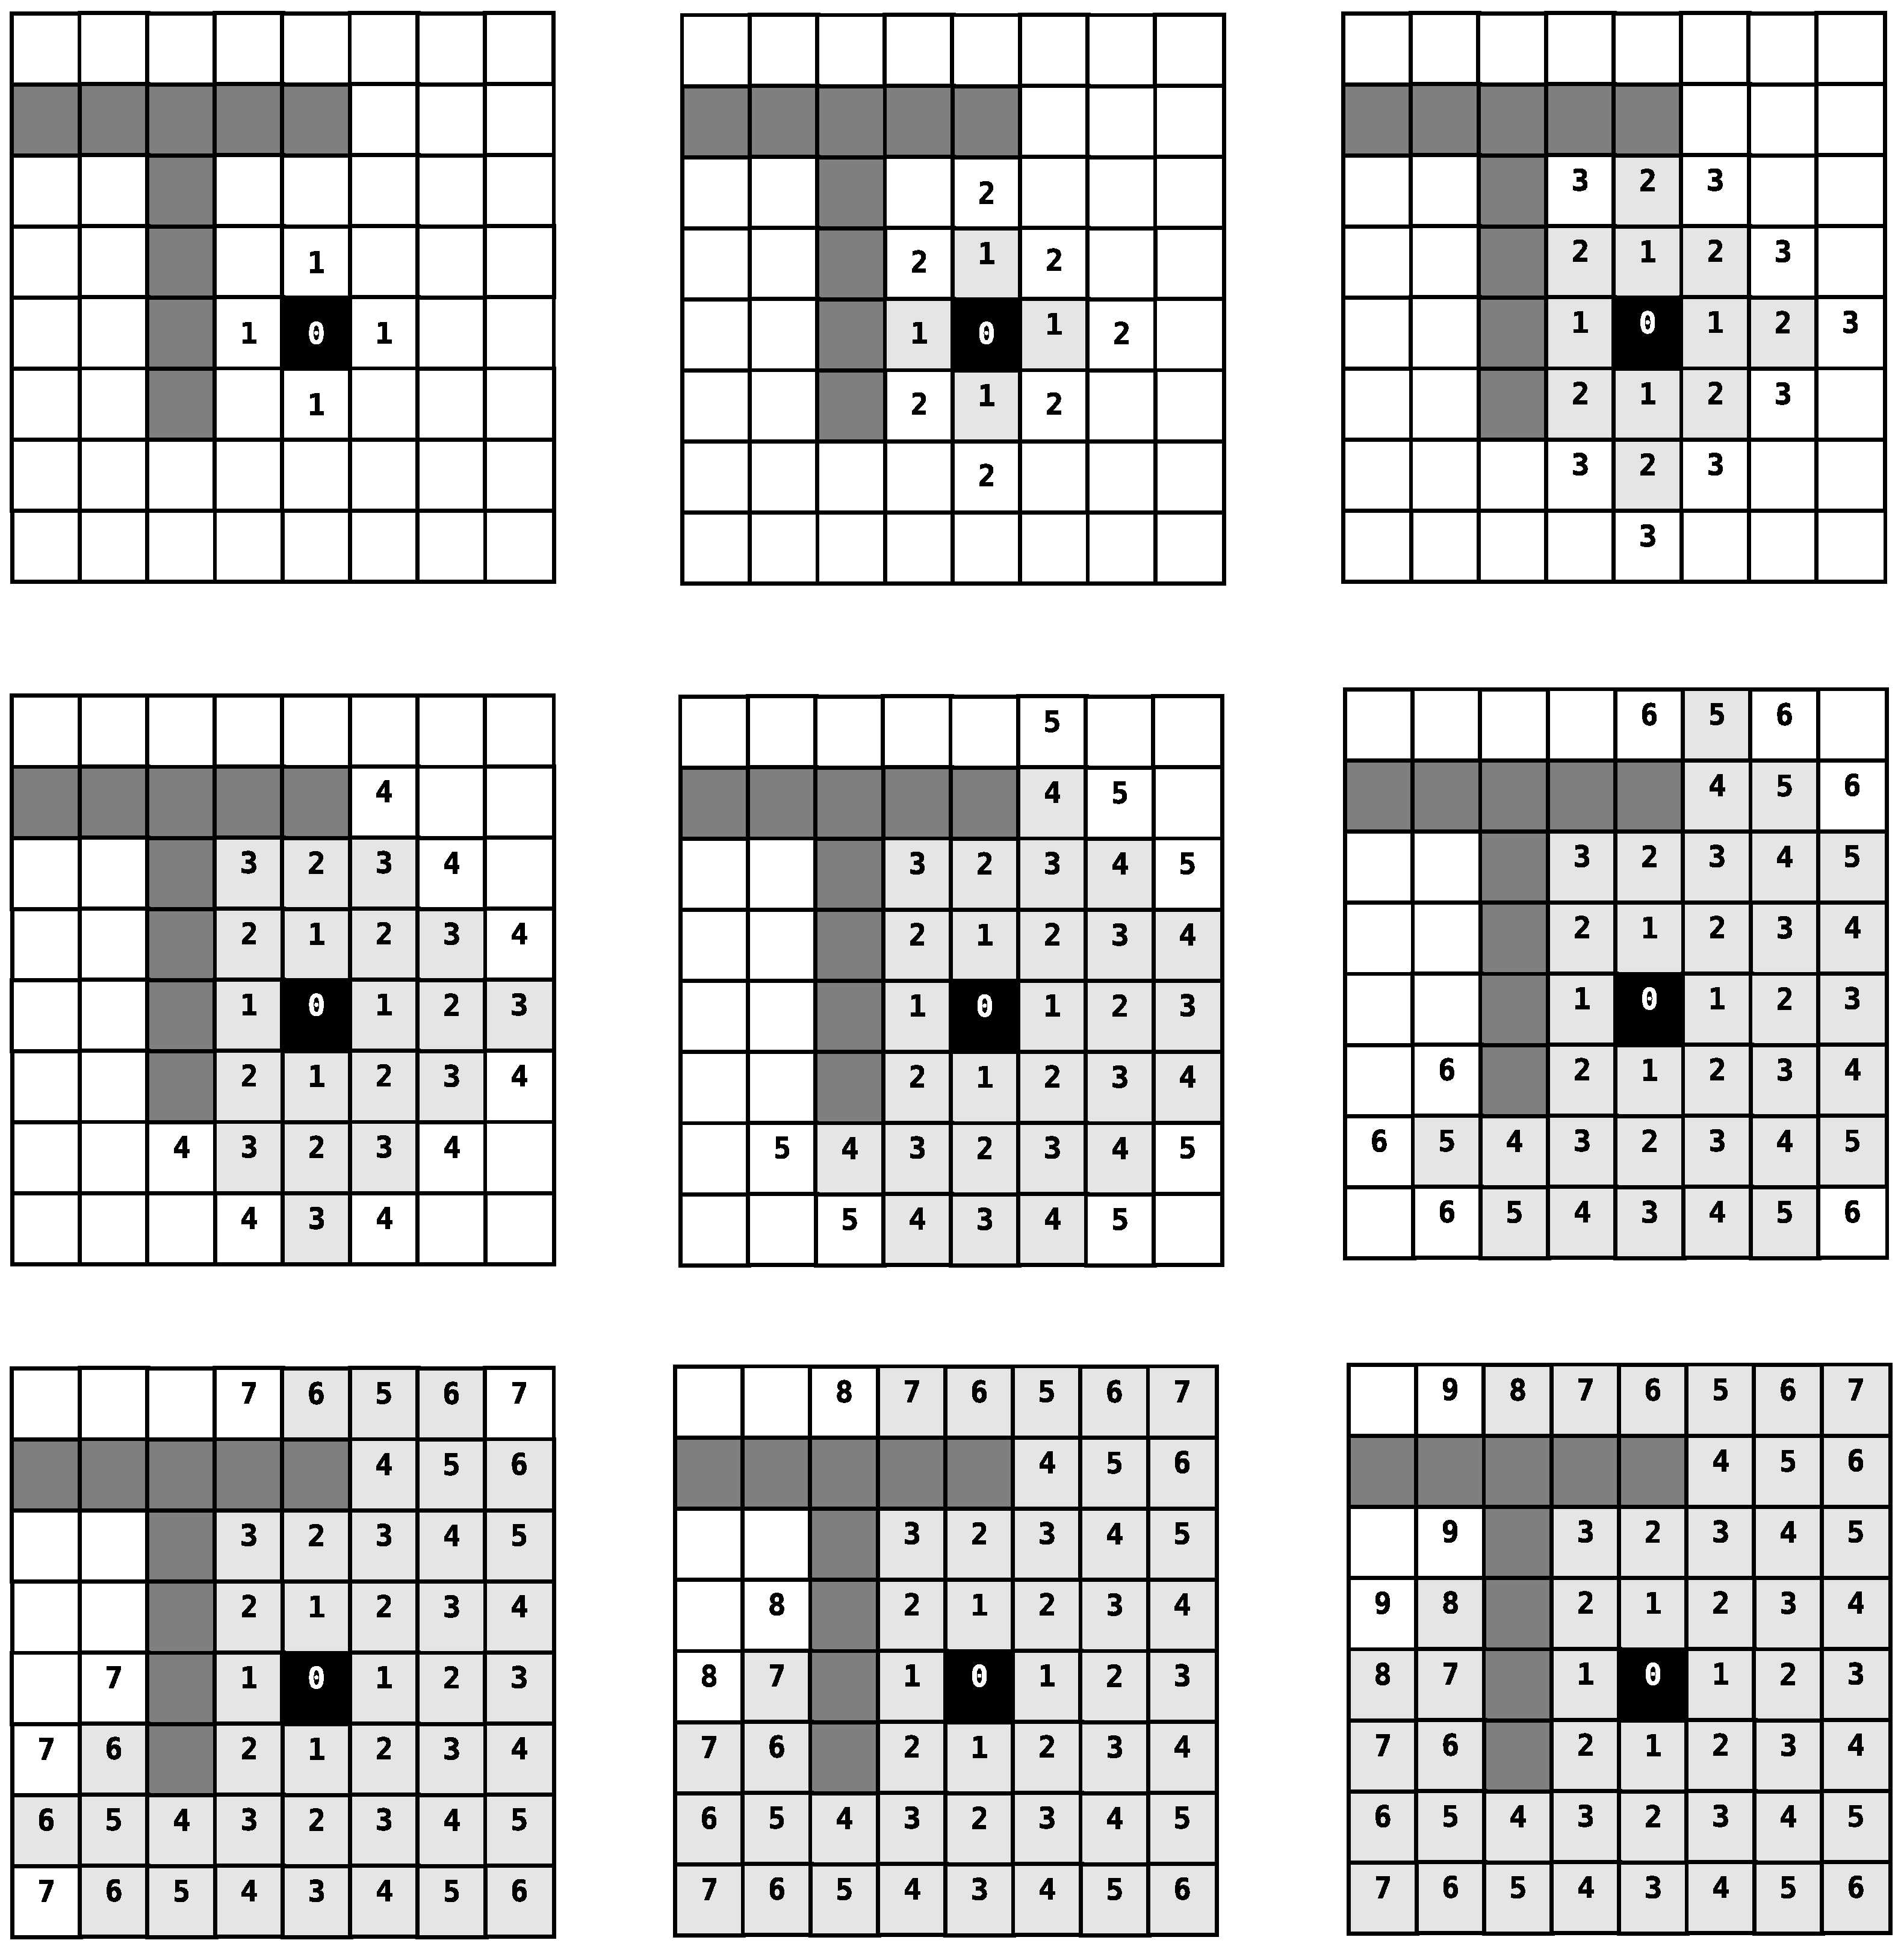
\includegraphics[height=0.9\textwidth]{algorithmik/flooding.eps}
\caption{Signalausbreitung eines Notausganges (Zelluläre Automaten)}
\label{fig:flooding}
\end{figure}

Die Signalausbreitung unterliegt dem lokalen Verhalten der zellulären Automaten durch die entsprechenden Zustandsübergangsregeln. Bei $i \geq 3$ Notausgängen sind die Zustandsübergangsregeln entsprechend komplex\footnote{Nach der Klassifizierung durch \cite{Wolfram} können die zellulären Automaten der Klasse 4 zugeordnet werden.} und werden an dieser Stelle nicht detailliert beschrieben.

\subsection{Orientierung der Personen bei der Flucht}

Nachdem die Signalausbreitung abgeschlossen ist, orientiert sich eine Person bei der Flucht anhand der lokalen Signal-Dämpfungswerten der aktuellen Zelle und der benachbarten Zellen. Das Bewegungsmodell wurde bereits in Abschnitt \ref{sec:bewegungsmodell} angeschnitten. Abbildung \ref{fig:fleeing} dient daher als visuelle Unterstützung der Fluchtwegbestimmung.

Zum Zeitpunkt $t_{-1}$ detektiert die Person eine Gefahrensituation. Die Person hat, über die \emph{Multilateration Lokalisierung} und der Kommunikation der Notausgänge, den Notausgang auf  $z_{exit} \in Z$ als nächstes verfügbares Evakuierungsziel bestimmt.

Die Person sei bei $t_{0}$ auf Zelle $z_{0} \in Z$ positioniert. Die Nachbarschaft sei mit $N_{Moore}(z_{0}) = Z_{z_{0}}$ gegeben. Anders als bei der Signalausbreitung bestimmt die Person den Fluchtweg über die Moore-Nachbarschaft. Der Vorteil liegt in der Möglichkeit diagonale Bewegungen auszuführen.

Die Ziel-Zelle $z_{i} \in Z$ für den nächsten Zeitschritt $t_{i}$  bestimmt die Person mittels der Funktion $N_{i}(Z_{z_{i-1}})$. Die Funktion $SN(z)$ liefert den Signal-Dämpfungswert einer Zelle.

\begin{quote}
$N_{i}(Z_{z_{i-1}}) \mathrel{\mathop:}= min(SN(z_{0_{u}})) = z_{i},$   $u = 1,...,\mid Z_{z_{i}}\mid$
\end{quote}

Entsprechend der Abbildung \ref{fig:fleeing} bestimmt die Person $t_{1}$, $t_{2}$ und $t_{3}$ folgende Ziel-Zellen:

\begin{quote}
($t_{1}$) $z_{1} = N_{1}(Z_{z_{0}}) = min(5,4,3,4, \infty , \infty , \infty , 6)$. $SN(z_{1}) = 3$\\

($t_{2}$) $z_{2} = N_{2}(Z_{z_{1}}) = min(\infty ,2,1,2,3,4,5,4)$. $SN(z_{2}) = 1$\\

($t_{3}$) $z_{3} = N_{3}(Z_{z_{2}}) = min(1,0,1,2,3,2,3,2)$. $SN(z_{3}) = 0$
\end{quote}

Erreicht eine Person eine Zelle mit dem Signal-Dämpfungswert $= 0$, versucht sie sich zu retten. Ist das Limit des Notausgangs bereits erreicht, sodass dieser blockiert, sucht sich die Person den nächstgelegenen verfügbaren Notausgang. Dafür ist eine Überlagerung der Signale von Notausgängen notwendig. Hinzu kommt die benötigte Verbindung zu einem verfügbaren Notausgang oder einer weiteren Person mit dem Wissen über einen verfügbaren Notausgang. Diese beiden Kriterien müssen erfüllt sein, sodass der Algorithmus zur Fluchtwegbestimmung funktioniert.

%Einteilung[Bearbeiten]
%
%Stephen Wolfram definiert in A New Kind of Science und in etlichen Arbeiten aus der Mitte der 1980er-Jahre vier Klassen, in die man die zellulären Automaten (genauer: die Regeln, die sie abarbeiten) je nach ihrem Verhalten unterteilen kann. Frühere Autoren versuchten lediglich, die Art der Muster für bestimmte Vorschriften zu ermitteln.
%Dem Aufwand nach geordnet waren dies die Klassen:
%Klasse 1: Fast alle ursprünglichen Muster entwickeln sich schnell zu einem stabilen und homogenen Zustand. Dadurch verschwindet jede Zufälligkeit in den ersten Mustern.
%Klasse 2: Fast alle ursprünglichen Muster entwickeln sich schnell in stabile oder oszillierende Strukturen. Einige Zufälligkeiten der ersten Muster kann man herausfiltern, jedoch können manche zurückbleiben. Lokale Änderungen am ursprünglichen Muster neigen dazu lokal zu bleiben.
%Klasse 3: Fast alle ursprünglichen Muster entwickeln sich pseudozufällig oder chaotisch. Jede stabile Struktur kann schnell durch Rauschen zerstört werden. Lokale Änderungen am ursprünglichen Muster neigen dazu, sich bis ins Unendliche auszubreiten.
%Klasse 4: Fast alle ursprünglichen Muster entwickeln sich in Strukturen, die vielschichtig und interessant interagieren. Endlich informative Ursprungsmuster können, wie in Klasse 2 üblich, stabile oder oszillierende Strukturen ergeben, aber die Anzahl der erforderlichen Schritte, um diesen Zustand zu erreichen, kann selbst für einfache Muster sehr groß sein. Lokale Änderungen am ursprünglichen Muster können sich bis ins Unendliche verbreiten.
%Wolfram hat vermutet, dass nicht alle zellulären Automaten der Klasse 4 dazu imstande sind, universelle Berechnungen auszuführen. Die Universalität hat sich vor allem für die Regel 110 und Conways Spiel des Lebens bestätigt.
%
%
%
%
%
%
%Die Von-Neumann-Nachbarschaft ist eine Nachbarschaftsbeziehung in einem quadratischen Raster. Lediglich die Flächen, welche eine Kante mit der Basisfläche gemeinsam haben, gelten als Nachbarn.
%Sie wurde nach John von Neumann benannt und wird auch als 4er-Nachbarschaft (bzw. Turmnachbarschaft aufgrund der Analogie zum Schach) bezeichnet.
%
%
%Die Moore-Nachbarschaft ist eine Nachbarschaftsbeziehung in einem quadratischen Raster. Alle Flächen, welche mindestens eine Ecke mit der Basisfläche gemeinsam haben, gelten als Nachbarn.
%Sie wurde nach Edward F. Moore benannt und wird auch als 8er-Nachbarschaft bezeichnet.




%Es gibt nur endlich viele Transitionsfunktionen f¨ur eine gegebene Zellenaufteilung.
%Bei n Nachbarn und k Farben gibt es nur kn+1 verschiedene Ausgangssituationen
%und k verschiedene Funktionswerte. Entsprechend ergeben sich daraus kkn+1
%verschiedene Transitionsfunktionen und damit zellul¨are Automaten.
%Entsprechend gibt es nur 223 = 256 verschiedene elementare zellul¨are Automaten.

\chapter{Evaluation}
\label{cha:evaluation}
%Eine Evaluation bzgl. Kommunikationsreichweiten, Anzahl „Agenten“ im Gebäude, oder Zeit bis zu vollständiger Evakuierung, etc. soll durchgeführt werden. Insbesondere sollte in der Evaluie-rung auf die Qualität der Lokalisierung in Abhängigkeit der Anzahl Notausgänge / Anchor Nodes, Anzahl Sensorknoten und der Kommunikationsreichweite eingegangen werden. 

\subsection{Lokalisierung}

Um die beste Lokalisierung mit dem Algorithmus zu erreichen, spielen die Parameter die größte Rolle. In den folgenden Tabellen und Analysen wird deutlich, wie groß die Unterschiede zwischen den verschiedenen Ausführungen sein kann, wenn man einen Parameter ein wenig verschiebt.

\paragraph{Beschreibung der Parameter und Tabellenspalten}



\begin{table}[h]
\begin{tabular}{|c|c|c|c|c|c|c|c|c|}
\hline
\textbf{No} & \textbf{\#Exits} & \textbf{\#Person} & \textbf{detRad} & \textbf{\#iter} & \textbf{~dist} & \textbf{avgDist} & \textbf{minDist} & \textbf{maxDist} \\ \hline
1           & 3                & 100               & 50              & 5               & 15             & 52               & 10               & 126              \\ \hline
2           & 3                & 100               & 50              & 5               & 30             & 35               & 3                & 115              \\ \hline
3           & 3                & 100               & 50              & 5               & 35             & 38               & 3                & 121              \\ \hline
4           & 3                & 100               & 50              & 10              & 15             & 52               & 10               & 126              \\ \hline
5           & 3                & 100               & 50              & 10              & 30             & 34               & 4                & 105              \\ \hline
6           & 3                & 100               & 50              & 10              & 35             & 28               & 1                & 109              \\ \hline
7           & 3                & 100               & 50              & 20              & 15             & 52               & 10               & 126              \\ \hline
8           & 3                & 100               & 50              & 20              & 30             & 33               & 4                & 90               \\ \hline
9           & 3                & 100               & 50              & 20              & 35             & 22               & 1                & 82               \\ \hline
10          & 3                & 100               & 50              & 30              & 15             & 52               & 10               & 126              \\ \hline
11          & 3                & 100               & 50              & 30              & 30             & 33               & 4                & 80               \\ \hline
12          & 3                & 100               & 50              & 30              & 35             & 20               & 1                & 66               \\ \hline
\end{tabular}
\end{table}

\subsection{Evakuierungsdauer}

Anzahl Notausgänge\\
20 Durchläufe\\
Zeit bis erste Person evakuiert\\
Zeit bis letzte Person evakuiert\\


\section{Effizienz}

\section{Fazit}

\section{Ausblick}

\subsubsection{Alternativer Orientierungsalgorithmus}
\label{sec:bug-0}
Als alternativer Orientierungsalgorithmus zur lokalen Fluchtwegfindung kann der \emph{Bug-0-Algorithmus} dienen.



%\appendix
%\chapter{Anhang}




% Literaturverzeichnis
\clearpage
\setcounter{page}{1}
\pagenumbering{roman}

\begin{thebibliography}{123}

\bibitem[1]{Amundson.}
Isaac Amundson and Xenofon D. Koutsoukos.
\newblock {\em {A} Survey on {L}ocalization for {M}obile {W}ireless {S}ensor {N}etworks}.
\newblock Department of Electrical Engineering and Computer Science, Vanderbilt University.


\bibitem[2]{Jonathan.2004}
{Jonathan Bachrach}, {Radhika Nagpal}, {Michael Salib} and {Howard Shrobe}.
\newblock {\em {E}xperimental {R}esults for and {T}heoretical {A}nalysis of a {S}elf-{O}rganizing {G}lobal {C}oordinate {S}ystem for {A}d {H}oc {S}ensor {N}etworks}.
\newblock Telecommunication Systems, page 213--233. 2004.

\bibitem[3]{Netlogo.1999}
Uri Wilensky.
\newblock {\em Netlogo}. 
\newblock Center for Connected Learning and Computer-Based Modeling, Northwestern University, Evanston, IL. 1999.
\newblock \url{http://ccl.northwestern.edu/netlogo/}, Stand: 26.01.2014.

\end{thebibliography}

\addtocontents{toc}{\protect\vspace*{\baselineskip}}
\addcontentsline{toc}{chapter}{Literaturverzeichnis}

\end{document}
